% Manuscript v10 | 2026-09-29 | Both DNA properties at t>=0.3, the setpoint sign rule and its probe, and a first compiled-LaTeX pass.
% Tables between DATA markers are regenerated by tools/build_results.py.
\documentclass{article}
\PassOptionsToPackage{numbers,compress}{natbib}
\usepackage[final,main]{neurips_2026}
\usepackage[utf8]{inputenc}
\usepackage[T1]{fontenc}
\usepackage{amsmath,amssymb,booktabs,graphicx,microtype,url}
\usepackage{algorithm,algpseudocode}
\usepackage{xcolor,tikz}
\usetikzlibrary{arrows.meta,positioning}
\usepackage{hyperref}
\hypersetup{hidelinks,pdftitle={BDG: Batch-Dispersion Guidance for Property-Band Generation},pdfsubject={Manuscript v10, 29 September 2026}}
\newcommand{\Fbar}{\bar F}
\newcommand{\Vb}{V_b}
\newcommand{\weff}{w_{\mathrm{eff}}}
\newcommand{\IB}{\mathrm{IB}}
\newcommand{\sg}{\operatorname{stopgrad}}
\title{BDG: Batch-Dispersion Guidance for\\Property-Band Generation}
\author{Bobo Li, Henry Huang\\
Department of Computer and Information Science, University of Pennsylvania\\
\small Manuscript v10 \quad 29 September 2026}
\begin{document}
% MAIN_TEXT_START
\maketitle
\begin{abstract}
Property-targeted generation must land inside a tolerance band while preserving sample quality. Standard gradient guidance scales target centering and distribution contraction together through a single strength. We introduce Batch-Dispersion Guidance (BDG), which sets the deviation coefficient from the batch endpoint variance relative to a requested variance while retaining the centering coefficient, at the same neural cost as plug-in guidance. We study two state spaces: QM9 molecules in Euclidean coordinates and DeepFlyBrain regulatory DNA on a probability simplex. A trained flow-matching model reaches 39.7 percent molecular stability against 28.8 for our variance-preserving diffusion model, so we carry flow matching forward, and plug-in guidance raises dipole coverage by 2.75 points on it. Across two flow backbones and three molecular properties, contracting BDG raises mean decoded coverage over plug-in by 0.45 to 1.52 points in all six comparisons and lowers mean absolute target error in every one, though the gains stay below our pre-registered threshold. A 612-cell ablation isolates gain, setpoint and strength, and shows monotone spread adjustment with a sign reversal about the setpoint. Transfer to DNA is property-dependent, not uniform: BDG gains 7.08 points on GC once the guidance window starts early enough to separate the baselines, while on CpG it gives up 4.88 because the plug-in baseline already contracts past the tightest setpoint our grid offers; an exploratory setpoint inside that spread recovers a 2.28-point gain, as the rule predicts. Hamming diversity changes little throughout; fidelity costs depend on the property and the window.
\end{abstract}

\section{Introduction}
Diffusion and flow matching generate structured samples by reversing corruption or learning transport velocities \citep{karras2022elucidating,lipman2022flow}. Comparing them on one task grounds the choice of generator in measured quality and cost \citep{albergo2025stochastic}.

Gradient guidance moves properties toward a target, but its strength also contracts their spread \citep{chung2023dps,song2023lgd}. Batch interactions and moment constraints motivate a separate dispersion setting \citep{corso2024particle,mgd2026moment}. Can this setting improve band coverage at an acceptable quality cost?

We compare linear FM and VP diffusion on QM9, then test BDG against plug-in and recent adaptations before transfer to DeepFlyBrain DNA. Our hypothesis is that a scalar property-dispersion rule adjusts coverage across different state spaces.\footnote{Code, evaluation cells and the scripts that regenerate every table: \url{https://github.com/Henry1145141919810/cis6270-project1-group2}}
Our contributions are summarized as follows.
\begin{itemize}
\item We select FM from a trained-model quality comparison.
\item We derive BDG's zero-gain limit and expansion condition.
\item We isolate gain, setpoint and strength in 612 ablation cells.
\item We quantify coverage, quality and cost across two modalities.
\end{itemize}
\section{Related Work}
\textbf{Continuous generation.} FM fits transport velocities; VP diffusion predicts corruption noise. Stochastic interpolants connect these formulations \citep{lipman2022flow,albergo2025stochastic}.

\textbf{Dispersion and guidance.} Particle Guidance introduces batch interactions \citep{corso2024particle}; Moment Guided Diffusion imposes moment constraints \citep{mgd2026moment}; variance tilting favors feature spread \citep{vtd2026variance}. BDG adds a batch variance residual to endpoint guidance, distinct from per-sample, uncertainty and Monte Carlo corrections. We claim this composition without distributional guarantees.

\textbf{Molecules.} Equivariant diffusion and EquiFM model molecular geometry \citep{hoogeboom2022equivariant,song2023equifm}.

\textbf{The comparators we measure.} All arms share one frozen backbone, sampler, seed set and evaluator, so only the steering rule varies. \emph{Plug-in} (DPS) differentiates a Gaussian likelihood at the endpoint estimate and is the common ancestor of the rest \citep{chung2023dps}. \emph{TMPD} divides it by an uncertainty denominator $s^2+v_f$ \citep{boys2024tmpd}; \emph{LGD-MC} averages plug-in gradients over draws scaled by the same variance \citep{song2023lgd}; \emph{TFG-MC} keeps TFG's Monte Carlo smoothing with a tuned scale and is not the full update \citep{ye2024tfg}. BDG instead reads a \emph{batch} statistic: the two uncertainty-based rules collapse to plug-in wherever residual endpoint variance vanishes, and BDG does not.

\textbf{Sequences.} Dirichlet FM and Fisher Flow model simplex-valued sequences; MOG-DFM guides discrete biological sequences \citep{stark2024dirichlet,davis2024fisher,chen2025multi}. Our measured sequence comparators are ports of the guidance rules above, not reproductions of these three generators.

\section{Methods}
\subsection{The Two Modalities, and How We Model Each}\label{sec:data}
The two state spaces are genuinely different, which is what makes transfer a test, not a change of dataset.

\textbf{QM9 molecules} are unordered atom sets: continuous coordinates in $\mathbb R^3$ plus one-hot H/C/N/O/F, padded with an atom-count mask $M$, and invariant to rotation and translation. We model them with an E(3)-equivariant graph network so that symmetry holds by construction. Decoding reads atom types and infers bonds from distances, so samples can be chemically \emph{invalid}, which we measure. Targets are $\mu$, $\alpha$ and the HOMO--LUMO gap.

\textbf{DeepFlyBrain DNA} is a 500-bp sequence written as 500 points on $\Delta^3$, so the state $(\Delta^3)^{500}$ is bounded and convex with data at its vertices; the relaxation adds an interior to move through. We model it with a dilated 1-D CNN and project back to the simplex at every Euler step. Decoding is per-position $\arg\max$, so \emph{every} sample is a legal sequence and quality must be judged by sequence statistics, not validity. Targets are GC, affine in the relaxed state, and CpG, quadratic.

Both generators are property-unconditional, so all targeting happens at sampling time. Splits, preprocessing and predictor pairs are in Appendix~\ref{app:data}; architectures and training in Appendix~\ref{app:training}.

\subsection{Continuous Flow Matching Baseline}\label{sec:fm}
With Gaussian source $x_0$, data $x_1$ and uniform $t\in[0,1]$, we train
\begin{equation}
x_t=(1-t)x_0+tx_1,\qquad \mathcal L_{\rm FM}=\mathbb E\|v_\theta(x_t,t;M)-(x_1-x_0)\|_M^2.
\label{eq:fm}
\end{equation}
The 3.75M-parameter EGNN (8 layers, width 256) uses Adam, batch 256, rate $2\times10^{-4}$, cosine decay and EMA 0.9999. Epoch-1500 EMA sampling uses 100 Euler steps (Table~\ref{tab:training}).

\subsection{Diffusion Baseline}\label{sec:diff}
Our trained VP model uses the same representation and EGNN configuration. For corruption time $u$, $a(u)=\exp[-(0.1u+9.95u^2)/2]$ and $\sigma^2(u)=1-a^2(u)$:
\begin{equation}
x_u=a(u)x_1+\sigma(u)\epsilon,\qquad\mathcal L_{\rm VP}=\mathbb E\|\epsilon_\phi(x_u,u;M)-\epsilon\|_M^2.
\label{eq:vp}
\end{equation}
Sampling integrates $\mathrm dx/\mathrm du=-\frac12\beta(u)(x-\epsilon_\phi/\sigma)$ backward, with $\beta(u)=0.1+19.9u$, 100 steps and terminal denoising. We evaluate the selected epoch-1475 EMA checkpoint.

\subsection{Guided Generation}\label{sec:guidance}
The frozen guide evaluates $F_i=f_A(m_i)$ at $m_i=x_t^{(i)}+(1-t)v_\theta(x_t^{(i)},t;M)$. Let $s$ be the calibration-pool property standard deviation. For target $y$, plug-in guidance adds
\begin{equation}
G_i=\frac{y-F_i}{s^2}\nabla_{x_t^{(i)}}F_i,\qquad
C_i=\operatorname{clip}_{\|v_i\|}\!\left[w\frac{1-t}{\max(t,\varepsilon)}G_i\right].
\label{eq:plug}
\end{equation}
On QM9 we apply $C_i$ for $t\ge0.5$, then mask and recenter molecular coordinates. The derivative includes the generator's endpoint Jacobian. All model weights stay frozen.

\subsection{Proposed Innovation: Batch-Dispersion Guidance}\label{sec:bdg}
For $B>1$, define $\Fbar=B^{-1}\sum_iF_i$, $\Vb=(B-1)^{-1}\sum_i(F_i-\Fbar)^2$, gain $\eta\ge0$ and setpoint $\tau=\tau_m s>0$. BDG replaces $y-F_i$ by
\begin{equation}
\begin{aligned}
n_i&=(y-F_i)-\eta e(F_i-\Fbar)=(y-\Fbar)-\weff(F_i-\Fbar),\\
e&=(\Vb-\tau^2)/\tau^2,\qquad \weff=1+\eta e.
\end{aligned}\label{eq:bdg}
\end{equation}
BDG retains the centering coefficient and detaches $n_i/s^2$ before pullback. \textbf{At $\eta=0$, BDG equals plug-in}; $\tau=0$ is undefined. Since $V_b\ge0$, $\weff\ge1-\eta$. Negative $e$ weakens contraction; expansion requires $\weff<0$, hence $\eta>1$. Terminal spread is not guaranteed (Algorithm~\ref{alg:bdg}).

\subsection{Transfer to Modality 2}\label{sec:transfer}
The sequence generator learns a linear path from Dirichlet$(1,1,1,1)$ noise to one-hot data, and BDG reads analytic soft GC and CpG properties, not a learned predictor, so the guided and scored quantities differ only by decoding. The dispersion rule itself is unchanged from Modality 1: only the state, the property and the decoder differ. Architecture, training length and checkpoint selection are in Appendix~\ref{app:training}; the simplex sampler and its soft/decoded property gap are in Appendix~\ref{app:m2}.

\subsection{Model Overview}\label{sec:overview}
Figure~\ref{fig:overview} separates training, frozen guidance and decoding across the two state spaces.
\begin{figure}[!t]
\centering
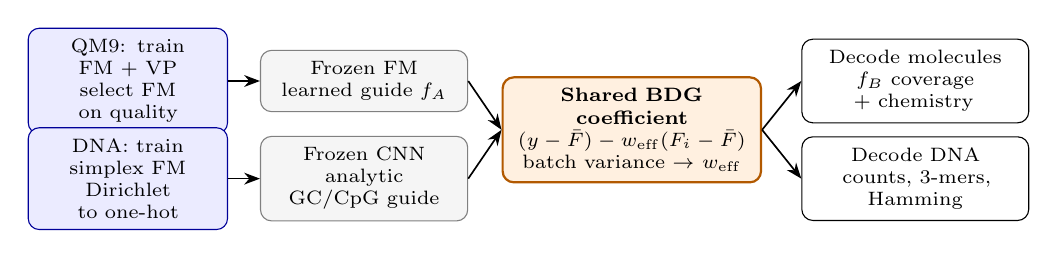
\begin{tikzpicture}[font=\scriptsize,
box/.style={draw,rounded corners,align=center,inner sep=4pt},
train/.style={box,fill=blue!8,draw=blue!60!black},
frozen/.style={box,fill=black!4,draw=black!50},
new/.style={box,fill=orange!12,draw=orange!70!black,thick},
arr/.style={-{Stealth},semithick}]
\node[train,text width=2.25cm] (fm) at (0,0.62) {QM9: train FM + VP\\select FM on quality};
\node[frozen,text width=2.35cm] (frozen) at (3,0.62) {Frozen FM\\learned guide $f_A$};
\node[new,text width=3.0cm] (bdg) at (6.4,0) {\textbf{Shared BDG coefficient}\\$(y-\Fbar)-\weff(F_i-\Fbar)$\\batch variance $\rightarrow\weff$};
\node[train,text width=2.25cm] (seq) at (0,-0.62) {DNA: train simplex FM\\Dirichlet to one-hot};
\node[frozen,text width=2.35cm] (sf) at (3,-0.62) {Frozen CNN\\analytic GC/CpG guide};
\node[box,text width=2.6cm] (eval1) at (10,0.62) {Decode molecules\\$f_B$ coverage + chemistry};
\node[box,text width=2.6cm] (eval2) at (10,-0.62) {Decode DNA\\counts, 3-mers, Hamming};
\draw[arr] (fm)--(frozen); \draw[arr] (seq)--(sf);
\draw[arr] (frozen.east)--(bdg.west); \draw[arr] (sf.east)--(bdg.west);
\draw[arr] (bdg.east)--(eval1.west); \draw[arr] (bdg.east)--(eval2.west);
\end{tikzpicture}
\caption{Training (blue), frozen components (gray), and shared BDG rule (orange). The state, guide and decoder change across modalities; the scalar dispersion rule is unchanged.}
\label{fig:overview}
\end{figure}

\section{Results}
\subsection{Evaluation Protocol}\label{sec:protocol}
\subsubsection{Metrics}
Targets are training medians (q50). Molecular IB counts decoded samples within $\delta=2\operatorname{MAE}_{\rm cal}(f_B)$ of $y$, accompanied by stability, validity and distinct-valid yield. DNA counts exact GC/CpG with half-widths 0.008833/0.008818, plus 3-mer JSD and Hamming diversity. Figure~\ref{fig:distributions} shows training distributions, q50 and both band rules. Coverage comparisons stay within matched tasks.
\subsubsection{Fair Comparison and Computational Budget}
Settings use three seeds, 2,000 samples each, batches of 500 and 100 Euler steps. Headline BDG uses $\eta=4$, $w=1$; ablations and DNA also use $w=4$. DNA reports the registered $t\ge0.5$ window and a $t\ge0.3$ follow-up covering both properties at $w\in\{1,4\}$; windows are never pooled (Appendix~\ref{app:evaluation}).
\subsubsection{Statistical Reporting}
Tables show mean $\pm$ seed sd. Molecular comparisons use unpaired binomial $|z|\ge2.99$ (18 contrasts, family level 0.05), ignoring batch coupling and rerun noise (Table~\ref{tab:contrasts}). Original DNA uses an exploratory $z=3.16$ threshold for 32 contrasts; the new window is descriptive.

\subsection{Modality 1: Flow Matching versus Diffusion}\label{sec:fmvd}
FM's higher stability (39.7\% versus 28.8\%) and validity (75.6\% versus 66.2\%) than our VP diffusion justify carrying it forward (Table~\ref{tab:fmvd}). Pretrained EquiFM (flow matching) also exceeds EDMsecond (diffusion) on these metrics. Our models share data, architecture and training settings; selection differs (Appendix~\ref{app:training}). External checkpoints provide supporting context.
% BEGIN DATA BASE
\begin{table}[!htbp]
\centering\small
\caption{Unguided QM9, $3\times2{,}000$ samples: percentages, mean $\pm$ seed sd. Lower rows use pretrained external models. Timing includes scoring: RTX A6000 except $^*$B200 MIG; runtimes are not hardware matched. Bold marks the best entry of each panel in each marked column and underline the runner-up; panels are ranked separately because their rows are not comparable across panels, a column is marked only where one direction is better, and a tie is left unmarked.}
\label{tab:fmvd}
\begin{tabular}{lccccc}
\toprule
Generator & Mol. stable$\uparrow$ & Valid$\uparrow$ & Unique$\uparrow$ & NFE & s/sample\\
\midrule
FM, ours & $\mathbf{39.7\pm0.6}$& $\mathbf{75.6\pm1.1}$& \underline{99.8}& 100 & 0.051\\
VP diffusion, ours & $\underline{28.8\pm1.3}$& $\underline{66.2\pm0.7}$& \textbf{99.9}& 101 & 0.048$^{*}$\\
\midrule
EquiFM (flow) & $\mathbf{86.2\pm0.3}$& $\mathbf{93.8\pm0.6}$& \underline{99.7}& 100 & 0.086\\
EDMsecond (diffusion) & $\underline{67.2\pm1.3}$& $\underline{86.0\pm1.3}$& \textbf{99.8}& 101 & 0.087\\
\bottomrule
\end{tabular}
\end{table}
% END DATA BASE

\subsection{Modality 1: Guided versus Unguided Generation}\label{sec:guidworks}
Plug-in raises decoded dipole/gap coverage by 2.75/2.35 points on FM and 2.13/2.60 on VP, all above threshold; both $\alpha$ changes remain unresolved. Stability falls by 4.08/6.15 points on FM and 2.68/5.65 on VP (Tables~\ref{tab:recent}, \ref{tab:full-vp}). Guidance therefore improves targeting on both families with a chemistry cost (Table~\ref{tab:guidance}).

% BEGIN DATA GUIDANCE
\begin{table}[!htbp]
\centering\small\setlength{\tabcolsep}{4pt}
\caption{Guided versus unguided under matched settings, $w=1$, $t\ge0.5$, three seeds of 2,000. Plug-in guidance is compared with the same frozen backbone and sampler. IB is decoded coverage (percent mean $\pm$ seed sd); $\Delta$ is percentage points. Stability and validity are reported so guidance is not judged by coverage alone. Bold marks the largest coverage gain and underline the runner-up.}
\label{tab:guidance}
\begin{tabular}{llccccccc}
\toprule
Backend & Prop. & IB un. & IB g. & $\Delta$IB & Stab. un. & Stab. g. & Val. un. & Val. g.\\
\midrule
FM, ours & $\mu$ & $7.8\pm0.1$ & $10.6\pm0.4$ & \textbf{+2.75}& 39.7 & 35.6 & 75.6 & 72.5\\
FM, ours & $\alpha$ & $5.0\pm0.3$ & $6.1\pm0.3$ & +1.07 & 39.7 & 37.2 & 75.6 & 73.7\\
FM, ours & gap & $10.3\pm1.0$ & $12.6\pm0.7$ & +2.35 & 39.7 & 33.6 & 75.6 & 69.9\\
\midrule
VP diffusion, ours & $\mu$ & $8.7\pm0.8$ & $10.8\pm0.4$ & +2.13 & 28.8 & 26.2 & 66.2 & 61.8\\
VP diffusion, ours & $\alpha$ & $5.2\pm0.6$ & $5.4\pm0.4$ & +0.15 & 28.8 & 25.2 & 66.2 & 58.7\\
VP diffusion, ours & gap & $9.8\pm0.6$ & $12.4\pm1.2$ & \underline{+2.60}& 28.8 & 23.2 & 66.2 & 57.3\\
\bottomrule
\end{tabular}
\end{table}
% END DATA GUIDANCE

\subsection{Modality 1: Innovation Ablations}\label{sec:ablations}
Table~\ref{tab:ablation} removes BDG's residual ($\eta=0$), changes its setpoint and increases plug-in strength. Contracting BDG improves dipole target concentration; increasing $\tau_m$ widens spread past unguided, which neither tested plug-in strength reaches (Figure~\ref{fig:results}a). The 612-cell grid and descriptive quality-cost comparisons appear in Appendix~\ref{app:ablations} and Table~\ref{tab:exchange}.
% BEGIN DATA ABLATION
\begin{table}[!htbp]
\centering\small
\caption{Dipole ablation on our FM: q50 $y=2.4932$ D, band $\pm0.17541$ D. IB is percent mean $\pm$ seed sd; stability is percent mean. Decoded MAE, mean and spread $\sigma$ are in D. Zero gain is plug-in; its $w=4$ row tests stronger guidance. $\tau_m$ is written -- at $\eta=0$, where $w_{\mathrm{eff}}=1$ and the setpoint has no effect. Coverage alone is not a quality ranking, and the quality columns show what each arm spent to reach it. Bold marks the best entry in each marked column and underline the runner-up; a column is marked only where one direction is better, and a tie is left unmarked, never broken arbitrarily.}
\label{tab:ablation}
\begin{tabular}{cccccccc}
\toprule
$w$ & $\eta$ & $\tau_m$ & IB$\uparrow$ & MAE$\downarrow$ & Mean & $\sigma$ & Stable$\uparrow$\\
\midrule
1 & 0 & -- & $10.6\pm0.4$ & 0.969 & 2.615 & 1.209 & 35.6\\
4 & 0 & -- & $\mathbf{13.4\pm0.4}$& \textbf{0.812}& 2.548 & 1.024 & 30.3\\
1 & 4 & 0.5 & $11.2\pm1.1$ & 0.903 & 2.609 & 1.113 & 35.1\\
1 & 4 & 1 & $8.9\pm0.2$ & 1.133 & 2.714 & 1.434 & \textbf{40.5}\\
1 & 8 & 0.5 & $\underline{11.9\pm0.3}$& \underline{0.861}& 2.603 & 1.064 & 34.0\\
1 & 8 & 1.5 & $7.6\pm0.2$ & 1.377 & 2.858 & 1.922 & \underline{37.6}\\
\bottomrule
\end{tabular}
\end{table}
% END DATA ABLATION

\subsection{Modality 1: Comparison with Recent Methods}\label{sec:recent}
At $\tau_m=0.5$, BDG improves mean coverage and MAE in all six flow/property comparisons, with higher seed variability on our FM and unresolved coverage gains. At $\tau_m=1$, spread increases and occupancy falls. BDG matches plug-in's neural calls and uses one fifth of LGD-MC/TFG's guide calls (Table~\ref{tab:cost}). TFG achieves higher coverage with greater stability loss (Tables~\ref{tab:recent}, \ref{tab:full-fm}--\ref{tab:full-edm}).
% BEGIN DATA M1
\begin{table}[!htbp]
\centering\small
\caption{Our FM, $w=1$: decoded IB, percent mean $\pm$ seed sd; stability means in $\mu/\alpha/\mathrm{gap}$ order. DV is distinct-valid yield (\%), and time is s/sample, both for $\mu$. Plug-in is $\eta=0$; BDG uses $\eta=4$. Rows are matched-backbone adaptations. Coverage alone is not a quality ranking, and the quality columns show what each arm spent to reach it. Bold marks the best entry in each marked column and underline the runner-up; a column is marked only where one direction is better, and a tie is left unmarked, never broken arbitrarily.}
\label{tab:recent}
\begin{tabular}{lcccccc}
\toprule
Method & IB $\mu\uparrow$ & IB $\alpha\uparrow$ & IB gap$\uparrow$ & Stable$\uparrow$ & DV$\uparrow$ & Time\\
\midrule
Unguided & $7.8\pm0.1$ & $5.0\pm0.3$ & $10.3\pm1.0$ & 39.7 / \textbf{39.7} / \textbf{39.7}& \underline{75.5}& \textbf{0.051}\\
Plug-in ($\eta=0$) & $10.6\pm0.4$ & $6.1\pm0.3$ & $12.6\pm0.7$ & 35.6 / 37.2 / 33.6& 72.4 & 0.119\\
TMPD-inspired & $9.0\pm0.6$ & $6.1\pm0.4$ & $11.6\pm0.9$ & 38.4 / 38.9 / 37.3& 74.7 & 0.255\\
LGD-MC & $9.6\pm0.8$ & $5.2\pm0.4$ & $10.8\pm0.7$ & \underline{39.9} / \underline{39.2} / \underline{39.5}& 75.4 & 0.229\\
TFG & $\mathbf{28.8\pm1.6}$& $\mathbf{10.5\pm0.3}$& $\mathbf{27.5\pm0.3}$& 24.5 / 26.8 / 14.4& 62.7 & 0.122\\
BDG, $\tau_m=0.5$ & $\underline{11.2\pm1.1}$& $\underline{7.0\pm0.5}$& $\underline{14.2\pm0.8}$& 35.1 / 36.4 / 30.0& 71.2 & 0.119\\
BDG, $\tau_m=1$ & $8.9\pm0.2$ & $5.6\pm0.5$ & $10.6\pm0.2$ & \textbf{40.5} / 37.9 / 37.6& \textbf{76.3}& 0.119\\
\bottomrule
\end{tabular}
\end{table}
% END DATA M1

\subsection{Modality 2: Transfer of the Innovation}\label{sec:m2}
Both properties now start guidance at $t=0.3$, where the four baselines separate; the original $t\ge0.5$ window, the only one giving identical plug-in/TMPD/LGD coverage, remains in Table~\ref{tab:m2-late}. At $w=4$ contracting BDG raises GC coverage from 30.25\% to 37.33\% (+7.08 points) but lowers CpG coverage from 91.51\% to 86.63\% ($-4.88$ points, Table~\ref{tab:m2}). One rule gives both signs. BDG servos batch spread to $\tau$, so it contracts only a batch wider than $\tau$: plug-in reaches $0.62s$ on GC, outside the $\tau_m=0.5$ setpoint, and $0.37s$ on CpG, already inside it, and BDG accordingly tightens GC to $0.59s$ and relaxes CpG to $0.45s$. Widening an over-contracted batch is the specified response, not a failed update, and $\tau_m=1$ relaxes both properties further (15.6\% and 54.3\%). What transfers is therefore the mechanism and its sign rule, not a coverage gain: the setpoint must sit below the baseline's achieved spread, and $\tau_m=0.5$ does so for only one of the two properties. Lowering the setpoint to $\tau_m=0.25$, inside CpG's achieved $0.372s$, does what the rule predicts: spread contracts to $0.298s$ and coverage returns to 93.73\%, $+2.28$ points over plug-in with all three seeds agreeing in sign, bought with a higher 3-mer JSD (Table~\ref{tab:setpoint}). That setpoint is outside our pre-registered grid, so it is an exploratory confirmation of the rule and not a headline number. Hamming diversity changes little.
% BEGIN DATA M2
\begin{table}[!htbp]
\centering\small\setlength{\tabcolsep}{3pt}
\caption{DNA, $w=4$, $t\ge0.3$ for both properties. IB is percent mean $\pm$ seed sd; JSD ($\times10^{-4}$), Hamming and s/sequence are GC/CpG. The original $t\ge0.5$ window, where the three uncertainty-based comparators are numerically indistinguishable from plug-in, is Table~\ref{tab:m2-late}. Coverage alone is not a quality ranking, and the quality columns show what each arm spent to reach it. Bold marks the best entry in each marked column and underline the runner-up; a column is marked only where one direction is better, and a tie is left unmarked, never broken arbitrarily.}
\label{tab:m2}
\begin{tabular}{lccccc}
\toprule
Method & GC IB$\uparrow$ & CpG IB$\uparrow$ & JSD$\downarrow$ & Hamming & Time\\
\midrule
Unguided & $14.0\pm1.0$ & $50.2\pm1.6$ & 4.53 / 4.53& 0.7456 / 0.7456 & \textbf{0.050} / \textbf{0.052}\\
DPS-style plug-in & $\underline{30.3\pm2.0}$& $\mathbf{91.5\pm0.5}$& 3.64 / 4.37& 0.7456 / 0.7455 & 0.124 / \underline{0.072}\\
TMPD-inspired & $29.2\pm2.1$ & $\underline{91.4\pm1.4}$& 3.66 / 4.36& 0.7455 / 0.7455 & 0.145 / 0.076\\
LGD-MC & $30.0\pm1.3$ & $90.7\pm0.6$ & 3.61 / 4.02& 0.7455 / 0.7454 & 0.131 / 0.109\\
TFG-MC adaptation & $29.8\pm1.8$ & $85.1\pm0.7$ & \textbf{3.57} / \textbf{3.56}& 0.7455 / 0.7454 & 0.109 / 0.122\\
BDG, $\tau_m=0.5$ & $\mathbf{37.3\pm6.5}$& $86.6\pm0.9$ & 4.24 / 3.94& 0.7455 / 0.7455 & 0.122 / 0.117\\
BDG, $\tau_m=1$ & $15.6\pm0.8$ & $54.3\pm0.6$ & \underline{3.59} / \underline{3.62}& 0.7455 / 0.7454 & \underline{0.075} / 0.115\\
\bottomrule
\end{tabular}
\end{table}
% END DATA M2
\begin{figure}[!t]
\centering
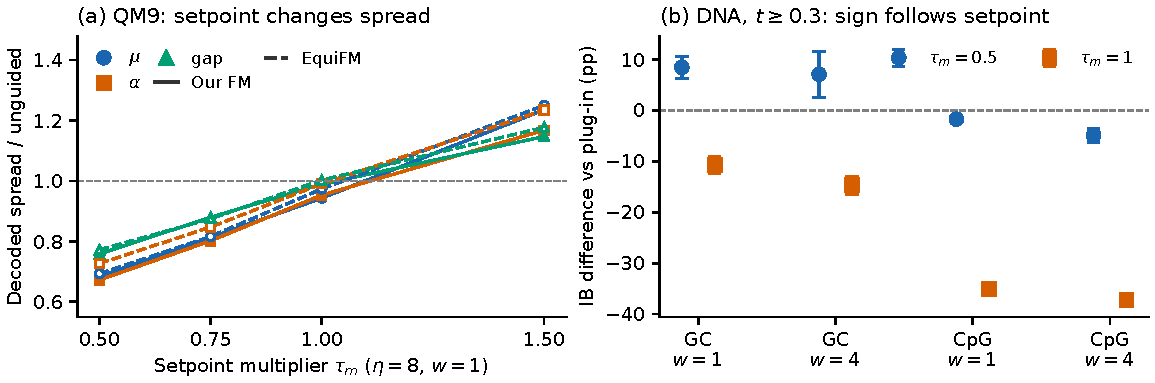
\includegraphics[width=\linewidth]{figs/results_v10.pdf}
\caption{(a) Decoded property spread relative to each backbone's unguided reference; points pool three seeds. Solid: our FM; dashed: EquiFM. (b) DNA coverage gain over plug-in, $\eta=4$; bars are sd of three paired seed differences. QM9 uses $t\ge0.5$. DNA uses $t\ge0.5$ except GC .3 ($t\ge0.3$); no $\tau_m=1$ cell was run there.}
\label{fig:results}
\end{figure}

\subsection{Cross-Modality Analysis and Failure Modes}\label{sec:failure}
BDG adjusts spread in both modalities, and on DNA the sign of its coverage effect is recovered from the setpoint alone: it helps where plug-in leaves the batch wider than $\tau$ and hurts where plug-in has already contracted past it (Appendix~\ref{app:m2}). GC baselines separate with earlier guidance, supporting a timing explanation for their late-window overlap.

\section{Discussion}
FM provides the stronger QM9 starting point; guidance improves targeting on both families. BDG adds adjustable spread and higher mean target concentration at plug-in's neural cost. TFG achieves more coverage with greater chemistry loss. DNA extends BDG to a second state space, where it gains on GC and loses on CpG exactly as its setpoint predicts.

The zero-gain and setpoint ablations connect BDG's added coefficient to decoded spread and occupancy. Retaining the centering term lets dispersion change without rescaling that coefficient; this does not imply independent mean dynamics or faster convergence.

Batch-aware intervals and joint in-band-and-stable yield would strengthen evaluation; fidelity-matched DNA comparisons would quantify the cost of the coverage each setpoint buys, and the exploratory $\tau_m=0.25$ probe that already recovers a CpG gain deserves a registered replication at both strengths. Matched-force comparisons and open-loop replay would test whether feedback itself is necessary. Next, control molecular atom counts more closely and define evaluation goals around the local property distribution near each target range, to address size and target-density confounding.
% MAIN_TEXT_END
\clearpage
\bibliographystyle{ieeetr}
\bibliography{citation,refs_extra}
\clearpage
\appendix
\renewcommand{\thetable}{S\arabic{table}}
\renewcommand{\theHtable}{S\arabic{table}}
\setcounter{table}{0}
\renewcommand{\thefigure}{S\arabic{figure}}
\renewcommand{\theHfigure}{S\arabic{figure}}
\setcounter{figure}{0}
\section{Reproducibility and Extended Results}
\subsection{Data Sources and Splits}\label{app:data}
QM9 uses the DeepChem/MoleculeNet packaging. The project retains the 3,054 entries excluded as uncharacterized in common EDM preprocessing, so published EDM dataset definitions are not identical. A seeded permutation creates the four splits stated in Section~\ref{sec:data}. Coordinates are centered, padded atoms are masked, and coordinates and one-hot features have no additional scaling. The E(3)-equivariant generator handles rotation and translation; invariant property predictors use training-derived normalization. Sample $i$ uses validation mask $i$ for $i=0,\ldots,1999$, identically across every arm, seed and backend. This fixed list has minimum 8, median 18, mean 17.87 and maximum 29 atoms. No histogram draw, size filtering or target-dependent size assignment occurs; all sizes receive the same q50 target. Seeds change initial noise only. No property label enters either generator.

DeepFlyBrain is the 500-bp enhancer data used by Dirichlet FM \citep{stark2024dirichlet}. Four ambiguous training examples were excluded from the supplied 83,726. The retained splits are 83,722/10,505/10,434; channels are A/C/G/T. Class labels are unused by our unconditional generator. These random-example splits do not test sequence-cluster generalization. The older 200-bp experiment is excluded.

Exact targets and calibration values are preserved in each source cell. Molecular band half-widths for our predictor pair are 0.17541 D for $\mu$, 0.50618 Bohr$^3$ for $\alpha$, and 0.00748 Ha for gap. External EquiFM uses a different predictor pair and therefore different acceptance widths. Its coverage must not be ranked directly against our FM's coverage.


\begin{figure}[!htbp]
\centering
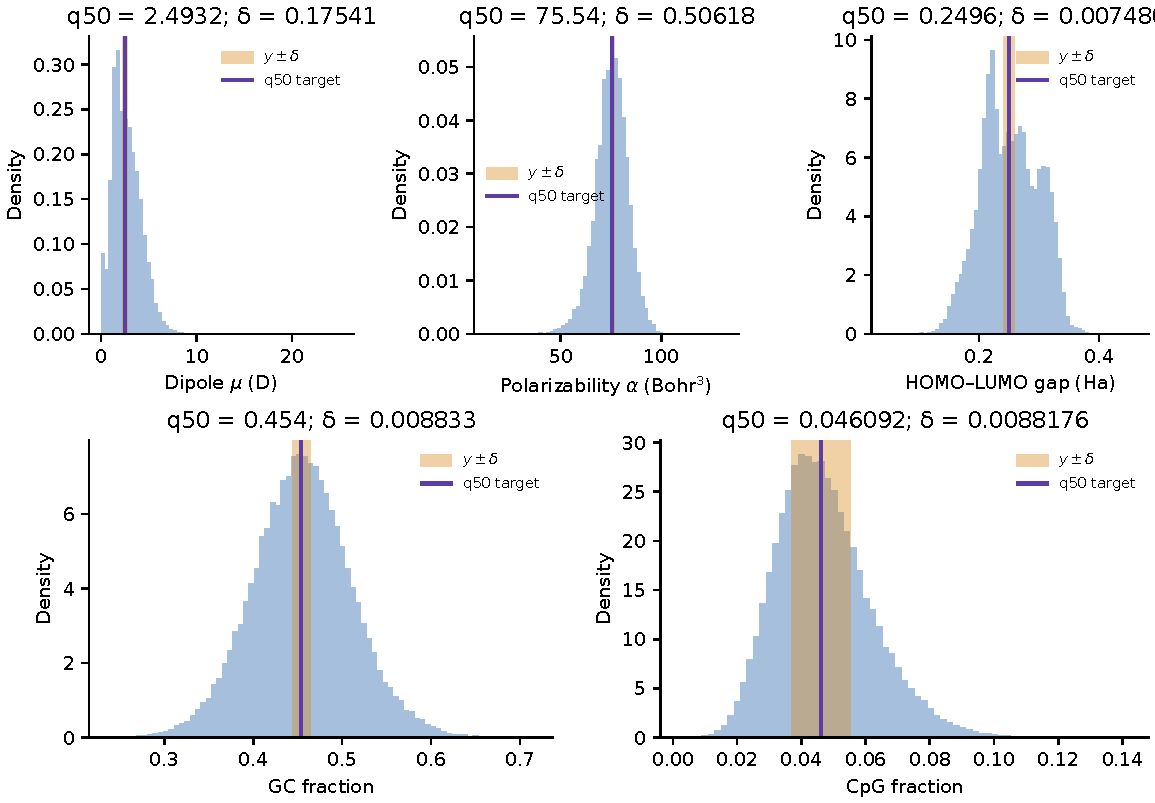
\includegraphics[width=\linewidth]{figs/property_distributions_v10.pdf}
\caption{Measured training-property distributions: QM9 train\_a (51,527 molecules, top) and DeepFlyBrain training (83,722 sequences, bottom). Purple marks q50 $y$; orange marks $[y-\delta,y+\delta]$. Histogram bins cover the full observed support. These are real-data reference distributions, not generated samples. QM9 bands shown use our predictor pair; EquiFM uses its separate calibrated bands.}
\label{fig:distributions}
\end{figure}
\noindent\textbf{Evaluation band versus controller setpoint.} For QM9,
\[
\delta=2\operatorname{MAE}_{\rm cal}(f_B)
=\frac{2}{|\mathcal C_B|}\sum_{j\in\mathcal C_B}|f_B(x_j)-y_j|.
\]
The internal evaluator is scored on calibration examples from train\_a, which it did not train on. For DNA, $\delta=\max(0.16s,4.4q)$, where $s$ is the training-property standard deviation and $q=1/500$ (GC) or $1/499$ (CpG). The lattice floor binds for CpG. Full bandwidth is $2\delta$; $\delta$ is fixed across guidance arms. BDG varies the requested spread $\tau=\tau_m s$, not the acceptance band.

\subsection{EGNN, Predictor Roles, and Molecular Decoding}\label{app:egnn}
EGNN stands for E(n)-Equivariant Graph Neural Network \citep{satorras2021egnn}. We implement its layers in plain PyTorch and train every internal generator and property network from scratch. EquiFM and EDM checkpoints are separate borrowed backends. Every distinct pair of real atoms is connected; padding and self-pairs are masked. E(n) includes rotations, reflections and translations. Distances are invariant, difference vectors transform with the molecule, and summing neighbours respects atom permutations. The scalar dipole magnitude is invariant; a dipole vector would rotate.

For atom features $h_i$, positions $x_i$ and $d_{ij}=\sqrt{\|x_i-x_j\|^2+10^{-8}}$, a layer computes
\begin{align*}
m_{ij}&=\phi_e(h_i,h_j,\|x_i-x_j\|^2),\\
h_i&\leftarrow h_i+\phi_h(h_i,\sum_j m_{ij}),\\
x_i&\leftarrow x_i+\sum_j (x_i-x_j)\phi_x(m_{ij})/(d_{ij}+1).
\end{align*}
Each $\phi$ is an MLP. Messages describe pairs, their sum updates features, and learned scalar weights move atoms along pair directions. One dense layer reaches all atoms; stacking layers learns richer interactions.

\texttt{EGNNVelocity} is the generator. Its input is noisy coordinates, continuous type channels, time and mask. Coordinate output is final minus initial position, recentered; a feature MLP returns type-channel output. FM reads these as velocities and VP as noise estimates. \texttt{EGNNScalar} keeps coordinates fixed, averages final features over real atoms, applies a pooling MLP, and uses a linear head for one property. Both $f_A$ and $f_B$ use this class with separate weights: $f_A$ steers predicted endpoints through the generator Jacobian; $f_B$ evaluates decoded samples and is absent from the guidance update. The training halves and calibration roles are disjoint as specified above.

For one molecule the FM error $z=v_\theta-v^*$ is $29\times8$: $z^c$ is $29\times3$ coordinate-velocity error and $z^f$ is $29\times5$ type-velocity error. Types remain continuous during noising and sampling; at the data endpoint they are one-hot H/C/N/O/F. Thus $v=(v^c,v^f)$ changes positions and type numbers. The loss masks padding and normalizes each part separately, as below.

\textbf{From cloud to molecule.} (1) The generator outputs real atom positions and five continuous type channels, with no bonds. (2) Argmax assigns the element: $[0.02,0.97,0.01,0,0.03]\mapsto$ C. (3) Pair distances in \AA\ are multiplied by 100 and compared with EDM's bond-length tables in pm, with margins 10/5/3 for single/double/triple bonds. For C--C, references are 154/134/120 pm: triple for $d<123$, double for $123\le d<139$, single for $139\le d<164$, and no bond otherwise. (4) Bond-order sums are checked against H:1, C:4, N:3, O:2, F:1; molecular stability requires all real atoms to pass. (5) RDKit builds atoms and bonds, sanitizes and canonicalizes SMILES. (6) Independently, $f_B$ scores final positions and argmax one-hot types for in-band membership; it does not consume the inferred bonds.

\subsection{Training and Checkpoint Records}\label{app:training}
Table~\ref{tab:training} records the training settings and evaluated checkpoints. For coordinates $c$, features $f$ and broadcast mask $M$, the training norm is
\[
\|z\|_M^2=\frac{\|M\odot z^c\|_2^2}{3\sum M}+\frac{\|M\odot z^f\|_2^2}{5\sum M}.
\]
Gaussian coordinate noise is centered; feature noise is independent Gaussian. Both molecular checkpoints specify the same split, architecture, optimizer, batch size, 1,500-epoch budget, EMA and training seed. The evaluated FM export is epoch-1500 EMA; VP is the selected epoch-1475 EMA, with validation loss 0.20784. The trainer selects validation atom stability with validation loss as a tie-breaker. The VP export records the selected epoch and configured budget, not proof of the final completed epoch. Consequently, Table~\ref{tab:fmvd} compares these trained checkpoints under shared settings with a disclosed selection difference; it does not establish family-wide superiority. VP training samples $u\in[10^{-3},1]$; its probability-flow ODE follows Equation~\eqref{eq:vp}.

\begin{table}[!htbp]
\centering\small
\caption{Training records and evaluated checkpoints. VP's selected epoch is 1475 within a configured 1500-epoch budget. Molecular predictors use one network per property and training half. Unrecorded training time is not inferred from sampling time.}
\label{tab:training}
\begin{tabular}{llll}
\toprule
Setting & Molecular FM / VP & $f_A$ / $f_B$ & Sequence FM\\
\midrule
Architecture & EGNN, 256, 8 layers & EGNN, 128, 4 & CNN, 128, 10\\
Parameters & 3.75M / 3.75M & 429,825 each & approximately 1.02M\\
Training data & \texttt{train\_a} & \texttt{train\_a}/\texttt{train\_b} & 83,722 sequences\\
Objective & velocity / noise MSE & property MSE & velocity MSE\\
Epoch budget & 1500 / 1500 & 120 & 1500 completed\\
Evaluated weights & EMA: 1500 / 1475 & validation checkpoint & epoch 1450\\
Batch size & 256 & 128 & 256\\
Optimizer & Adam & Adam & Adam\\
Initial learning rate & $2\times10^{-4}$ & $3\times10^{-4}$ & $2\times10^{-3}$\\
Schedule & cosine, floor 5\% & cosine & cosine to zero\\
EMA & 0.9999 & none & none\\
Training seed & 20260918 / 20260918 & 20260918 & 20260921\\
Training time & not fully recorded & not fully recorded & 539.7 min\\
\bottomrule
\end{tabular}
\end{table}

Sequence training performed 492,000 updates across 1,500 epochs. Validation selected update 475,600 (epoch 1450), loss 0.0633644, with 121.75M sample-views at the selected checkpoint. The total run lasted 539.7 minutes on RTX A6000, including validation. We distinguish completed training length from the selected checkpoint's age. The checkpoint uses Adam without EMA; its best-validation weights are sampled.

\begin{table}[!htbp]
\centering\small
\caption{Checkpoint fingerprints from the result records and local files. Prefixes identify artifacts; full hashes are retained in the source records.}
\label{tab:hashes}
\begin{tabular}{lll}
\toprule
Component & Identifier & Evidence\\
\midrule
Our molecular FM & MD5 \texttt{e19ccc06} & v3 cells, epoch 1500\\
Borrowed EDMsecond & MD5 \texttt{6abbd010} & v3 cells, released checkpoint\\
Sequence FM & MD5 \texttt{7f59b60b} & local checkpoint, best validation\\
Our VP diffusion & MD5 \texttt{8a3390a6} & v3 cells, epoch 1475\\
\bottomrule
\end{tabular}
\end{table}
Table~\ref{tab:hashes} identifies the evaluated artifacts. FM, EquiFM and EDMsecond cells record PyTorch 2.11.0+cu130, CUDA 13.0 and RTX A6000. VP cells record PyTorch 2.11.0+cu128, CUDA 12.8 and NVIDIA B200 MIG 2g.45gb. VP's local checkpoint MD5 matches every result cell. Hardware differs, so elapsed seconds cannot establish an FM--VP speed advantage. The sequence training report identifies RTX A6000, but individual sequence evaluation cells omit the device; those timings are not hardware-matched cross-modality benchmarks.

\subsection{Evaluation, Uncertainty, and Cost}\label{app:evaluation}
Molecular seeds are 20261001, 20261002 and 20261003. Sequence seeds are 20260921, 20260922 and 20260923. Each 2,000-sample cell contains four independent controller batches of size 500. Enlarging the total sample count adds batches, not observations to a single variance estimate. At fixed weights, seed variation measures sampling variation, not training uncertainty.

Molecular coverage counts decoded samples satisfying $|f_B(\hat x)-y|\le\delta$. Calibration uses 3,000 molecules drawn from the two training halves; each internal predictor is scored on the half it did not train on. The wrapper sets $s$ to the property standard deviation of this calibration pool, which differs from the raw predictor checkpoint's normalization scale. This $s$ sets the guidance energy and BDG setpoint; evaluator error sets $\delta$. Coverage on continuous features remains in source records but is not substituted for decoded IB.

Atom stability checks bond/valence rules; molecular stability requires every atom to pass. RDKit validity checks reconstruction and sanitization. Uniqueness divides distinct valid SMILES by valid samples; distinct-valid yield divides by all attempts. None is an energy or experimental viability measurement. IB includes invalid molecules, so usable yield requires the joint event of decoded in-band membership and stability. Marginal IB and stability cannot be multiplied to recover that event. The local aggregate results do not include the sample-level sidecars needed for this joint analysis.

The reported unpaired statistic is
\[
 z=\frac{p_a-p_b}{\sqrt{p_a(1-p_a)/6000+p_b(1-p_b)/6000}}.
\]
The registered molecular bar is 2.99. Table~\ref{tab:contrasts} reports the corresponding threshold-sized difference separately for every contrast; it is neither a power calculation nor evidence of equivalence. Within-batch dependence can invalidate an independent-Bernoulli variance, and common-noise pairing changes covariance. We retain this protocol statistic with explicit limitations and show seed standard deviations. A batch-aware paired bootstrap would need the sample-level records. At $\tau_m=0.5$, all six molecular coverage differences favor BDG in their means but remain below this bar. At $\tau_m=1$, three differences cross the bar against BDG and three remain unresolved. These outcomes distinguish an occupancy-setting effect from a universal coverage improvement. DNA uses the rule only as an exploratory comparison, and the stated positive effects survive the 32-contrast threshold of 3.16. For selections from the full molecular grid, the protocol's adjusted bar is 3.49; the paper makes descriptive grid claims without converting them into headline tests.

EquiFM same-seed reruns differ by up to 0.007 in continuous coverage. Its $\eta=0$ control agrees with plug-in only to the rerun tolerance, not bitwise. Our FM reproduces exactly. EDMsecond has same-seed variation up to 0.0015 in molecular stability. Neither binomial errors nor three seed values fully characterize this extra implementation variability.

The molecular run contains 162 headline cells, including 18 from our VP diffusion model, and 612 ablation cells. Summed recorded wall-clock is 16.77 hours for headline and 65.15 for ablations, 81.92 total. VP contributes 0.813 hours on different hardware. The original DNA files contain 84 headline, 111 ablation/window and four single-seed strength cells (199 files, 5.26 recorded hours). The window and setpoint follow-ups add 105 files: 96 at $t_{\min}=0.3$ (eight arms, three seeds, both properties, $w\in\{1,4\}$), four single-seed $t_{\min}=0.2$ probes, and five setpoint-probe cells. The $t_{\min}=0.2$ and setpoint cells are exploratory, and of the latter only $\tau_m=0.25$ carries three seeds. The new files add 5.86 recorded hours, for 11.12 DNA hours in total. Twelve original configurations repeat across trees; zero-gain controls are reported separately. The repeated configurations are checked for agreement and never pooled as extra seeds. Concurrent cells and evaluation overhead prevent interpreting these totals as elapsed time or accelerator utilization.

NFE counts solver field evaluations, distinct from generator forwards and derivative calls. For each molecular flow batch, plug-in and BDG record 200 generator forwards, 50 generator VJPs, and 50 guide forward/backward pairs; unguided records 100 generator forwards. VP unguided sampling adds terminal denoising for 101 evaluations. Sequence plug-in/BDG batches record 150 generator forwards and 50 VJPs at $t\ge0.5$, or 170 forwards and 70 VJPs at $t\ge0.3$; both use 100 solver steps. BDG adds scalar reductions to plug-in, not another neural call. Equal calls do not imply equal measured runtime. Clip fractions divide clipped sample-steps by samples times guided steps \emph{per batch}; using the batch-summed step count understates them fourfold.

Table~\ref{tab:cost} separates the recorded operation types. BDG and plug-in share these counts, while LGD-MC and TFG use five times as many guide forward/backward calls. These counts describe the sampled configurations; neither derivative calls nor Monte Carlo calls are interchangeable units of runtime.
% BEGIN DATA COST
\begin{table}[!htbp]
\centering\small
\caption{Recorded sampling operations per 2,000-molecule cell, our FM, dipole, $w=1$. Forward calls, vector--Jacobian products (VJP) and Jacobian--vector products (JVP) are separate operations, not equal-cost units. Evaluator calls are outside these counts; Table~\ref{tab:recent} reports wall-clock including scoring. No entry is marked here: these counts are exact and fixed by construction, plug-in and both BDG rungs are identical by design, and the smallest entry in every column belongs to the unguided reference, which performs no guidance at all.}
\label{tab:cost}
\begin{tabular}{lccccc}
\toprule
Method & Gen. forward & Gen. VJP & Gen. JVP & Guide forward & Guide backward\\
\midrule
Unguided & 400 & 0 & 0 & 0 & 0\\
DPS-style plug-in & 800 & 200 & 0 & 200 & 200\\
TMPD-inspired & 800 & 200 & 200 & 200 & 200\\
LGD-MC & 800 & 200 & 200 & 1000 & 1000\\
TFG & 600 & 200 & 0 & 1000 & 1000\\
BDG, $\tau_m=0.5$ & 800 & 200 & 0 & 200 & 200\\
BDG, $\tau_m=1$ & 800 & 200 & 0 & 200 & 200\\
\bottomrule
\end{tabular}
\end{table}
% END DATA COST

\subsection{Full Molecular Comparisons}\label{app:comparisons}
Tables~\ref{tab:full-fm}, \ref{tab:full-equifm}, \ref{tab:full-edm} and~\ref{tab:full-vp} report every headline arm and property. All numbers are generated by this project; no published score is mixed into these rows. EquiFM uses the released TFG guide/evaluator pair; our FM, our VP diffusion and borrowed EDMsecond use our disjoint pair. External training overlap, architectures, scales and selection differ, so all guidance contrasts stay within a backend. Equal nominal strength exposes each adaptation's behavior under shared settings; it is not a ranking of separately optimized methods.

DPS-style plug-in adapts posterior guidance to a Gaussian property energy and a flow endpoint. TMPD-inspired guidance uses a linearized uncertainty correction; LGD-MC marginalizes a local property loss; TFG combines training-free corrections. The implementations retain the local endpoint, clipping and timing choices in the cell records, and are adaptations of the cited methods, not reproductions of every original experimental setting. Molecular TFG and sequence TFG-MC are different implementations; the latter omits full TFG's iterative schedule.
% BEGIN DATA FULL-FM
\begin{table}[!htbp]
\centering\small
\caption{Complete headline evaluation on our FM. IB is decoded; IB and stability show percent mean $\pm$ seed sd. Validity and distinct-valid yield (DV) are percentages; time is recorded cell wall-clock divided by attempts. $w=1$, $t\ge0.5$, three seeds, $n=2{,}000$ each. Bold marks the best entry of each panel in each marked column and underline the runner-up; panels are ranked separately because their rows are not comparable across panels, a column is marked only where one direction is better, and a tie is left unmarked.}
\label{tab:full-fm}
\begin{tabular}{llccccc}
\toprule
Property & Method & IB$\uparrow$ & Stable$\uparrow$ & Valid$\uparrow$ & DV$\uparrow$ & s/sample\\
\midrule
$\mu$ & Unguided & $7.8\pm0.1$ & $39.7\pm0.6$ & \underline{75.6}& \underline{75.5}& \textbf{0.051}\\
$\mu$ & DPS-style plug-in & $10.6\pm0.4$ & $35.6\pm0.3$ & 72.5 & 72.4 & 0.119\\
$\mu$ & TMPD-inspired & $9.0\pm0.6$ & $38.4\pm0.6$ & 74.8 & 74.7 & 0.255\\
$\mu$ & LGD-MC & $9.6\pm0.8$ & $\underline{39.9\pm0.3}$& 75.5 & 75.4 & 0.229\\
$\mu$ & TFG & $\mathbf{28.8\pm1.6}$& $24.5\pm1.0$ & 62.8 & 62.7 & 0.122\\
$\mu$ & BDG, $\tau_m=0.5$ & $\underline{11.2\pm1.1}$& $35.1\pm1.1$ & 71.4 & 71.2 & 0.119\\
$\mu$ & BDG, $\tau_m=1$ & $8.9\pm0.2$ & $\mathbf{40.5\pm0.8}$& \textbf{76.5}& \textbf{76.3}& 0.119\\
\midrule
$\alpha$ & Unguided & $5.0\pm0.3$ & $\mathbf{39.7\pm0.6}$& \textbf{75.6}& \textbf{75.5}& \textbf{0.050}\\
$\alpha$ & DPS-style plug-in & $6.1\pm0.3$ & $37.2\pm1.6$ & 73.7 & 73.6 & 0.118\\
$\alpha$ & TMPD-inspired & $6.1\pm0.4$ & $38.9\pm1.1$ & 75.1 & 75.0 & 0.200\\
$\alpha$ & LGD-MC & $5.2\pm0.4$ & $\underline{39.2\pm1.3}$& 74.9 & 74.9 & 0.224\\
$\alpha$ & TFG & $\mathbf{10.5\pm0.3}$& $26.8\pm0.8$ & 61.2 & 61.1 & 0.121\\
$\alpha$ & BDG, $\tau_m=0.5$ & $\underline{7.0\pm0.5}$& $36.4\pm1.0$ & 72.2 & 72.1 & 0.118\\
$\alpha$ & BDG, $\tau_m=1$ & $5.6\pm0.5$ & $37.9\pm1.1$ & 75.1 & \underline{75.1}& 0.118\\
\midrule
gap & Unguided & $10.3\pm1.0$ & $\mathbf{39.7\pm0.6}$& \textbf{75.6}& \textbf{75.5}& \textbf{0.051}\\
gap & DPS-style plug-in & $12.6\pm0.7$ & $33.6\pm0.8$ & 69.9 & 69.8 & 0.119\\
gap & TMPD-inspired & $11.6\pm0.9$ & $37.3\pm0.7$ & 73.8 & 73.7 & 0.201\\
gap & LGD-MC & $10.8\pm0.7$ & $\underline{39.5\pm0.8}$& \underline{75.2}& \underline{75.1}& 0.225\\
gap & TFG & $\mathbf{27.5\pm0.3}$& $14.4\pm0.8$ & 45.5 & 45.5 & 0.122\\
gap & BDG, $\tau_m=0.5$ & $\underline{14.2\pm0.8}$& $30.0\pm0.4$ & 65.8 & 65.7 & 0.119\\
gap & BDG, $\tau_m=1$ & $10.6\pm0.2$ & $37.6\pm0.8$ & 74.3 & 74.2 & 0.119\\
\bottomrule
\end{tabular}
\end{table}
% END DATA FULL-FM
\clearpage
% BEGIN DATA FULL-EQUIFM
\begin{table}[!htbp]
\centering\small
\caption{Complete headline evaluation on borrowed EquiFM. IB is decoded; IB and stability show percent mean $\pm$ seed sd. Validity and distinct-valid yield (DV) are percentages; time is recorded cell wall-clock divided by attempts. $w=1$, $t\ge0.5$, three seeds, $n=2{,}000$ each. Bold marks the best entry of each panel in each marked column and underline the runner-up; panels are ranked separately because their rows are not comparable across panels, a column is marked only where one direction is better, and a tie is left unmarked.}
\label{tab:full-equifm}
\begin{tabular}{llccccc}
\toprule
Property & Method & IB$\uparrow$ & Stable$\uparrow$ & Valid$\uparrow$ & DV$\uparrow$ & s/sample\\
\midrule
$\mu$ & Unguided & $8.7\pm0.8$ & $\mathbf{86.2\pm0.3}$& \textbf{93.8}& \textbf{93.5}& \textbf{0.086}\\
$\mu$ & DPS-style plug-in & $10.9\pm0.9$ & $82.1\pm0.7$ & 91.9 & 91.6 & \underline{0.231}\\
$\mu$ & TMPD-inspired & $9.0\pm0.3$ & $85.3\pm0.4$ & 93.5 & 93.2 & 0.366\\
$\mu$ & LGD-MC & $9.7\pm0.3$ & $85.5\pm0.4$ & 93.3 & 93.1 & 0.474\\
$\mu$ & TFG & $\underline{11.9\pm0.3}$& $74.0\pm0.7$ & 86.5 & 86.2 & 0.301\\
$\mu$ & BDG, $\tau_m=0.5$ & $\mathbf{12.1\pm0.5}$& $79.3\pm0.7$ & 90.9 & 90.6 & 0.232\\
$\mu$ & BDG, $\tau_m=1$ & $8.9\pm0.7$ & $\underline{85.8\pm0.3}$& \underline{93.6}& \underline{93.3}& 0.232\\
\midrule
$\alpha$ & Unguided & $2.1\pm0.1$ & $\mathbf{86.2\pm0.3}$& \textbf{93.8}& \textbf{93.5}& \textbf{0.087}\\
$\alpha$ & DPS-style plug-in & $2.1\pm0.2$ & $82.9\pm0.4$ & 91.9 & 91.7 & 0.233\\
$\alpha$ & TMPD-inspired & $2.1\pm0.3$ & $84.8\pm0.3$ & 93.3 & 93.0 & 0.368\\
$\alpha$ & LGD-MC & $2.1\pm0.1$ & $\underline{85.5\pm0.9}$& 93.3 & 93.0 & 0.476\\
$\alpha$ & TFG & $\mathbf{3.4\pm0.5}$& $64.5\pm0.5$ & 84.5 & 84.4 & 0.302\\
$\alpha$ & BDG, $\tau_m=0.5$ & $\underline{2.5\pm0.2}$& $76.6\pm0.5$ & 89.5 & 89.2 & 0.233\\
$\alpha$ & BDG, $\tau_m=1$ & $2.0\pm0.1$ & $84.8\pm0.5$ & 92.8 & 92.6 & 0.233\\
\midrule
gap & Unguided & $4.9\pm0.2$ & $\mathbf{86.2\pm0.3}$& \textbf{93.8}& \textbf{93.5}& \textbf{0.086}\\
gap & DPS-style plug-in & $5.9\pm0.3$ & $82.7\pm0.4$ & 91.9 & 91.7 & 0.231\\
gap & TMPD-inspired & $5.1\pm0.3$ & $84.6\pm0.7$ & 92.7 & 92.4 & 0.365\\
gap & LGD-MC & $5.1\pm0.4$ & $\underline{86.1\pm0.2}$& \underline{93.5}& \underline{93.3}& 0.473\\
gap & TFG & $\mathbf{10.9\pm0.2}$& $55.5\pm1.4$ & 76.4 & 76.2 & 0.300\\
gap & BDG, $\tau_m=0.5$ & $\underline{6.8\pm0.8}$& $77.4\pm1.1$ & 90.1 & 90.0 & 0.231\\
gap & BDG, $\tau_m=1$ & $5.0\pm0.4$ & $85.6\pm0.3$ & 93.4 & 93.1 & 0.231\\
\bottomrule
\end{tabular}
\end{table}
% END DATA FULL-EQUIFM
% BEGIN DATA FULL-EDM
\begin{table}[!htbp]
\centering\small
\caption{Complete headline evaluation on borrowed EDMsecond. IB is decoded; IB and stability show percent mean $\pm$ seed sd. Validity and distinct-valid yield (DV) are percentages; time is recorded cell wall-clock divided by attempts. $w=1$, $t\ge0.5$, three seeds, $n=2{,}000$ each. Bold marks the best entry of each panel in each marked column and underline the runner-up; panels are ranked separately because their rows are not comparable across panels, a column is marked only where one direction is better, and a tie is left unmarked.}
\label{tab:full-edm}
\begin{tabular}{llccccc}
\toprule
Property & Method & IB$\uparrow$ & Stable$\uparrow$ & Valid$\uparrow$ & DV$\uparrow$ & s/sample\\
\midrule
$\mu$ & Unguided & $\underline{9.4\pm0.2}$& $\mathbf{67.2\pm1.3}$& \textbf{86.0}& \textbf{85.8}& \textbf{0.087}\\
$\mu$ & DPS-style plug-in & $\mathbf{11.2\pm1.1}$& $\underline{62.2\pm0.6}$& \underline{82.8}& \underline{82.7}& \underline{0.210}\\
\midrule
$\alpha$ & Unguided & $\underline{5.4\pm0.7}$& $\mathbf{67.2\pm1.2}$& \textbf{86.0}& \textbf{85.8}& \textbf{0.087}\\
$\alpha$ & DPS-style plug-in & $\mathbf{6.1\pm0.4}$& $\underline{64.6\pm0.8}$& \underline{84.1}& \underline{83.9}& \underline{0.208}\\
\midrule
gap & Unguided & $\underline{10.8\pm0.7}$& $\mathbf{67.1\pm1.3}$& \textbf{86.0}& \textbf{85.8}& \textbf{0.087}\\
gap & DPS-style plug-in & $\mathbf{12.8\pm0.7}$& $\underline{57.9\pm1.7}$& \underline{80.3}& \underline{80.2}& \underline{0.209}\\
\bottomrule
\end{tabular}
\end{table}
% END DATA FULL-EDM
\clearpage
% BEGIN DATA FULL-VP
\begin{table}[!htbp]
\centering\small
\caption{Complete headline evaluation on our VP diffusion. IB is decoded; IB and stability show percent mean $\pm$ seed sd. Validity and distinct-valid yield (DV) are percentages; time is recorded cell wall-clock divided by attempts. $w=1$, $t\ge0.5$, three seeds, $n=2{,}000$ each. Bold marks the best entry of each panel in each marked column and underline the runner-up; panels are ranked separately because their rows are not comparable across panels, a column is marked only where one direction is better, and a tie is left unmarked.}
\label{tab:full-vp}
\begin{tabular}{llccccc}
\toprule
Property & Method & IB$\uparrow$ & Stable$\uparrow$ & Valid$\uparrow$ & DV$\uparrow$ & s/sample\\
\midrule
$\mu$ & Unguided & $\underline{8.7\pm0.8}$& $\mathbf{28.8\pm1.3}$& \textbf{66.2}& \textbf{66.1}& \textbf{0.048}\\
$\mu$ & DPS-style plug-in & $\mathbf{10.8\pm0.4}$& $\underline{26.2\pm0.9}$& \underline{61.8}& \underline{61.7}& \underline{0.114}\\
\midrule
$\alpha$ & Unguided & $\underline{5.2\pm0.6}$& $\mathbf{28.8\pm1.3}$& \textbf{66.2}& \textbf{66.1}& \textbf{0.048}\\
$\alpha$ & DPS-style plug-in & $\mathbf{5.4\pm0.4}$& $\underline{25.2\pm1.5}$& \underline{58.7}& \underline{58.6}& \underline{0.114}\\
\midrule
gap & Unguided & $\underline{9.8\pm0.6}$& $\mathbf{28.8\pm1.3}$& \textbf{66.2}& \textbf{66.1}& \textbf{0.048}\\
gap & DPS-style plug-in & $\mathbf{12.4\pm1.2}$& $\underline{23.2\pm0.6}$& \underline{57.3}& \underline{57.3}& \underline{0.114}\\
\bottomrule
\end{tabular}
\end{table}
% END DATA FULL-VP
% BEGIN DATA CONTRASTS
\begin{table}[!htbp]
\centering\small
\caption{BDG minus plug-in on decoded molecular IB. Differences, paired seed sd and the threshold-sized difference $2.99\,\mathrm{se}(\Delta)$ are in percentage points. The registered unpaired statistic is shown separately from descriptive pairing. Bold marks the best entry in each marked column and underline the runner-up; a column is marked only where one direction is better, and a tie is left unmarked, never broken arbitrarily. The test statistic and its threshold are left unmarked: ranking significance is not a comparison this protocol makes.}
\label{tab:contrasts}
\begin{tabular}{llccccc}
\toprule
Backend & Property & $\tau_m$ & $\Delta$IB & SD$(\Delta)$ & $z$ & Threshold\\
\midrule
fm & $\mu$ & 0.5 & +0.63 & 1.45 & +1.11 & 1.70\\
fm & $\mu$ & 1 & -1.68 & 0.19 & -3.11 & 1.62\\
fm & $\alpha$ & 0.5 & +0.90 & 0.50 & +2.00 & 1.35\\
fm & $\alpha$ & 1 & -0.43 & 0.75 & -1.01 & 1.28\\
fm & gap & 0.5 & \textbf{+1.52}& 0.21 & +2.44 & 1.86\\
fm & gap & 1 & -2.07 & 0.72 & -3.54 & 1.75\\
equifm & $\mu$ & 0.5 & \underline{+1.25}& 0.70 & +2.15 & 1.74\\
equifm & $\mu$ & 1 & -1.93 & 0.62 & -3.55 & 1.63\\
equifm & $\alpha$ & 0.5 & +0.45 & 0.13 & +1.65 & 0.81\\
equifm & $\alpha$ & 1 & -0.02 & 0.31 & -0.06 & 0.77\\
equifm & gap & 0.5 & +0.90 & 0.56 & +2.02 & 1.33\\
equifm & gap & 1 & -0.93 & 0.67 & -2.25 & 1.24\\
\bottomrule
\end{tabular}
\end{table}
% END DATA CONTRASTS

\subsection{Complete Molecular Ablation Grids}\label{app:ablations}
Figures~\ref{fig:abl-fm} and~\ref{fig:abl-equifm} show every nonzero gain/setpoint combination as decoded coverage change from its own zero-gain control, with strengths kept separate. Tables~\ref{tab:grid-fm-mu}, \ref{tab:grid-fm-alpha}, \ref{tab:grid-fm-gap}, \ref{tab:grid-equifm-mu}, \ref{tab:grid-equifm-alpha} and~\ref{tab:grid-equifm-gap} provide the complete numeric ablations: 204 configurations, each evaluated with three seeds, accounting for all 612 cells. Each caption specifies its property, q50 target and band. These tables extend the selected dipole rows in Table~\ref{tab:ablation} with both strengths, all gains and setpoints, target error, bias, spread and stability.

For our FM dipole task at $w=1$, zero gain gives MAE 0.969 D and pooled mean 2.615 D around $y=2.4932$ D. At $\tau_m=0.5$, gains 4 and 8 lower MAE to 0.903 and 0.861 D and move the mean to 2.609 and 2.603 D. This supports improved endpoint target concentration in the selected ablation. Mean bias is not uniformly improved across properties: our FM gap bias grows slightly in magnitude at gain 4 despite lower MAE. Increasing gain also need not monotonically increase coverage, especially at $w=4$. The wider setpoint lowers occupancy of the fixed band in every grid, illustrating the intended spread--occupancy trade-off.

At $\eta=8,w=1,\tau_m=1.5$, decoded spread exceeds unguided for all three properties and both flow backends, approximately 1.15--1.25 times the reference. The tested positive plug-in strengths $w\in\{1,4\}$ remain below it. This comparison does not exclude signed strengths, arbitrary schedules, or a shifted plug-in target from reaching similar states. One-sided residuals, open-loop replay and signed-strength controls were not part of the completed grid.

Across the four setpoints at $\eta=8,w=1$, all six decoded spread curves increase monotonically (Figure~\ref{fig:results}a). The step-averaged deviation coefficient and decoded coverage have Spearman correlations of 0.92--0.99 across the 16 nonzero configurations in each of the 12 fixed-backbone/property/strength grids. This descriptive association links coefficient changes to occupancy; it does not separate closed-loop feedback from guidance magnitude.

Table~\ref{tab:exchange} compares $\Delta\mathrm{IB}/(-\Delta\mathrm{stability})$, with both differences measured in percentage points from the same ablation-stage plug-in reference at $w=1$. Contracting BDG at $\eta=8$ gains more coverage per stability point lost than increasing plug-in strength to $w=4$ in five of six tasks; at the headline gain $\eta=4$, this holds in four of six. These exploratory ratios are sensitive to small denominators, do not establish statistical superiority, and are not joint in-band-and-stable yield. The full grid reports the underlying metrics.
% BEGIN DATA EXCHANGE
\begin{table}[!htbp]
\centering\small
\caption{Exploratory coverage gained per stability point lost. All differences use the ablation-stage zero-gain reference at $w=1$. BDG changes $\eta$ at $\tau_m=0.5,w=1$; the strength control keeps $\eta=0$ and increases $w$ to 4. Ratios use decoded IB and molecular stability means, not joint useful yield. Bold marks the best entry in each marked column and underline the runner-up; a column is marked only where one direction is better, and a tie is left unmarked, never broken arbitrarily.}
\label{tab:exchange}
\begin{tabular}{llccc}
\toprule
Backend & Property & BDG $\eta=4$ & BDG $\eta=8$ & Plug-in $w=4$\\
\midrule
Our FM & $\mu$ & \textbf{1.267}& \underline{0.792}& 0.534\\
Our FM & $\alpha$ & \textbf{1.174}& \underline{0.806}& 0.439\\
Our FM & gap & \underline{0.423}& \textbf{0.524}& 0.383\\
EquiFM & $\mu$ & \underline{0.370}& \textbf{0.385}& 0.369\\
EquiFM & $\alpha$ & 0.053 & \underline{0.057}& \textbf{0.083}\\
EquiFM & gap & 0.149 & \textbf{0.238}& \underline{0.217}\\
\bottomrule
\end{tabular}
\end{table}
% END DATA EXCHANGE
\begin{figure}[!htbp]
\centering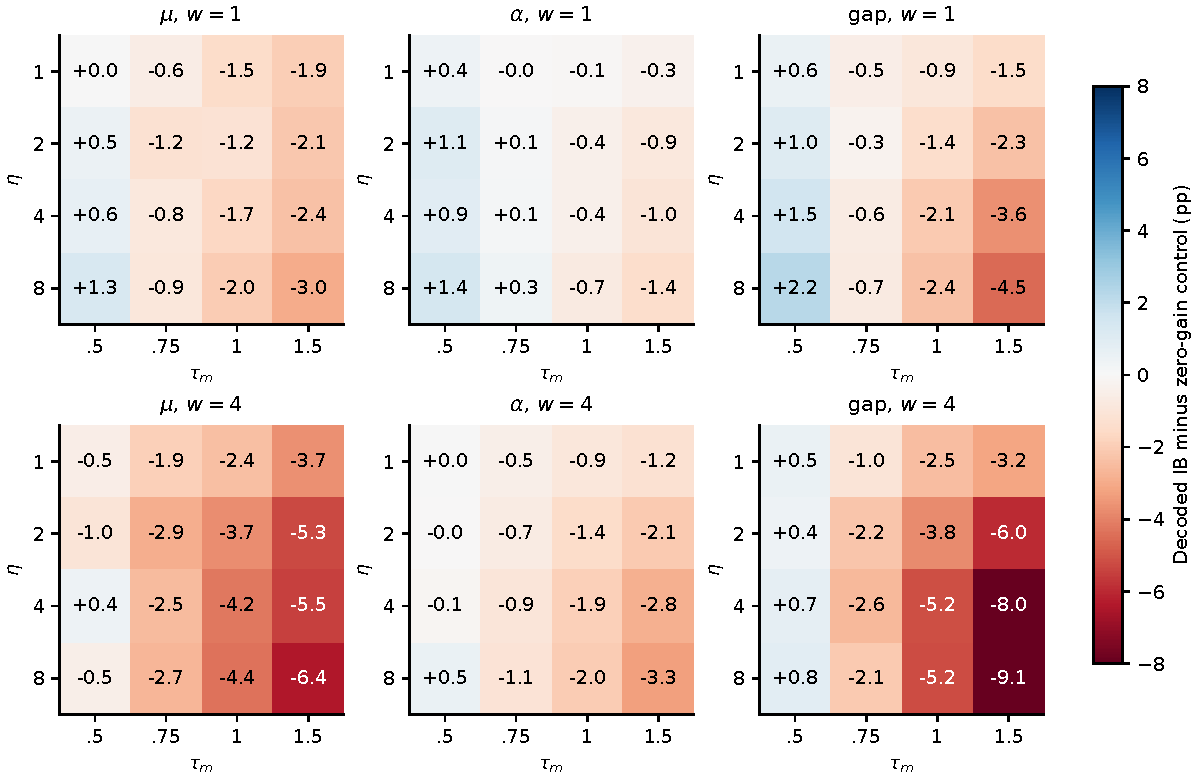
\includegraphics[width=\linewidth]{figs/ablation_fm_v10.pdf}
\caption{Our FM: full decoded coverage ablation. Each panel fixes property and strength; entries are percentage-point changes from $\eta=0$ at that strength. The color scale is shared with Figure~\ref{fig:abl-equifm}; values outside its range retain their exact text.}
\label{fig:abl-fm}
\end{figure}
\begin{figure}[!htbp]
\centering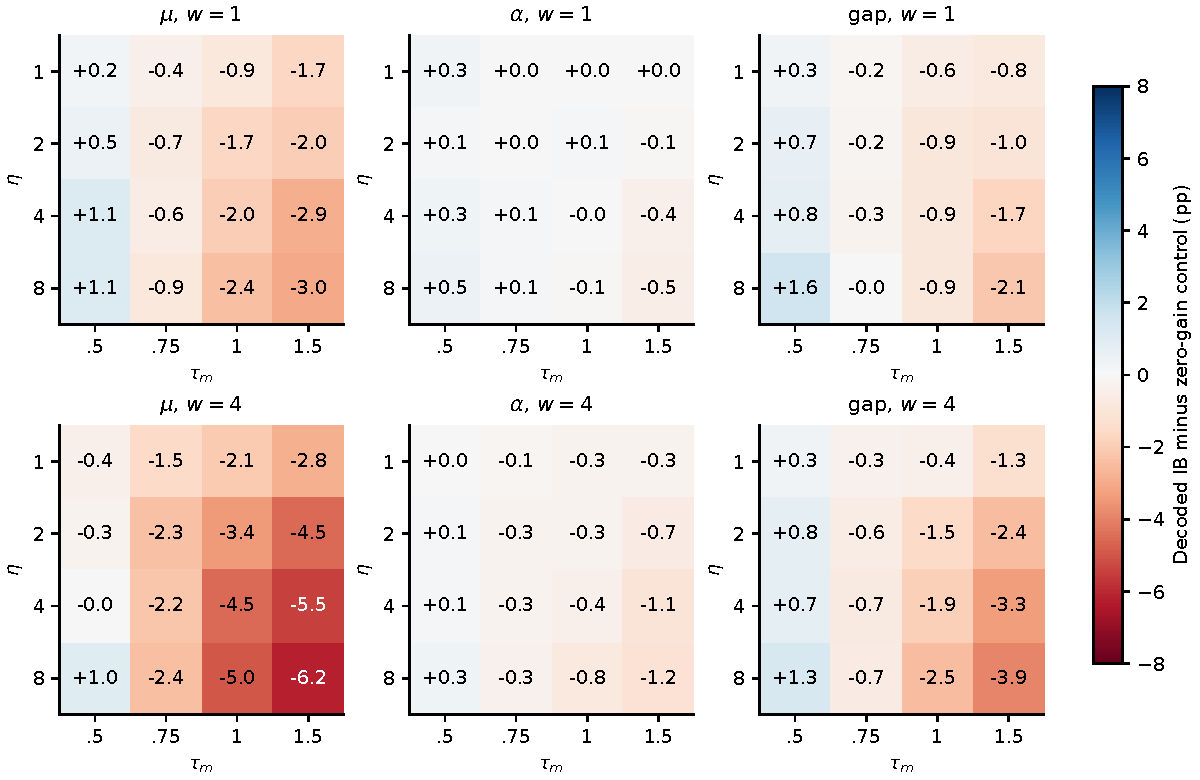
\includegraphics[width=\linewidth]{figs/ablation_equifm_v10.pdf}
\caption{Borrowed EquiFM: the same complete grid and matched zero-gain contrasts. Rerun variability accompanies the three-seed averages.}
\label{fig:abl-equifm}
\end{figure}
\clearpage
% BEGIN DATA GRID-FM-MU
\begin{table}[!htbp]
\centering\small
\caption{Our FM, $\mu$: all gain/setpoint ablations at $w=1,4$, q50 target $y=2.4932$ D, half-width $\delta=0.17541$ D. Each row uses three seeds of 2,000 samples. IB and molecular stability are percent mean $\pm$ seed sd. MAE, signed bias of the pooled mean, and pooled standard deviation $\sigma$ are decoded and normalized by $\delta$. The $\eta=0$ row removes the residual; its setpoint is irrelevant. Bold marks the best entry in each marked column and underline the runner-up; a column is marked only where one direction is better, and a tie is left unmarked, never broken arbitrarily.}
\label{tab:grid-fm-mu}
\begin{tabular}{cccccccc}
\toprule
$w$ & $\eta$ & $\tau_m$ & IB$\uparrow$ & MAE/$\delta\downarrow$ & Bias/$\delta$ & $\sigma/\delta$ & Stable$\uparrow$\\
\midrule
1 & 0 & -- & $10.6\pm0.4$ & 5.53 & +0.69 & 6.89 & $35.6\pm0.3$\\
1 & 1 & 0.5 & $10.6\pm0.2$ & 5.42 & +0.75 & 6.74 & $35.7\pm0.2$\\
1 & 1 & 0.75 & $10.0\pm0.0$ & 5.77 & +0.89 & 7.13 & $37.8\pm0.5$\\
1 & 1 & 1 & $9.1\pm0.1$ & 6.00 & +1.03 & 7.45 & $38.9\pm1.2$\\
1 & 1 & 1.5 & $8.6\pm0.2$ & 6.24 & +1.21 & 7.81 & $39.2\pm0.7$\\
1 & 2 & 0.5 & $11.1\pm0.5$ & 5.30 & +0.70 & 6.56 & $35.8\pm0.5$\\
1 & 2 & 0.75 & $9.4\pm0.3$ & 5.90 & +1.01 & 7.33 & $38.8\pm1.2$\\
1 & 2 & 1 & $9.4\pm0.4$ & 6.23 & +1.25 & 7.77 & $39.6\pm0.4$\\
1 & 2 & 1.5 & $8.5\pm0.5$ & 6.81 & +1.45 & 8.82 & $39.4\pm0.9$\\
1 & 4 & 0.5 & $11.2\pm1.1$ & 5.15 & +0.66 & 6.35 & $35.1\pm1.1$\\
1 & 4 & 0.75 & $9.8\pm0.5$ & 5.91 & +1.03 & 7.30 & $38.9\pm0.3$\\
1 & 4 & 1 & $8.9\pm0.2$ & 6.46 & +1.26 & 8.17 & $\mathbf{40.5\pm0.8}$\\
1 & 4 & 1.5 & $8.2\pm0.7$ & 7.27 & +1.71 & 9.93 & $38.2\pm1.0$\\
1 & 8 & 0.5 & $11.9\pm0.3$ & 4.91 & +0.62 & 6.07 & $34.0\pm0.5$\\
1 & 8 & 0.75 & $9.7\pm0.4$ & 5.82 & +1.02 & 7.21 & $38.7\pm0.5$\\
1 & 8 & 1 & $8.6\pm0.4$ & 6.64 & +1.37 & 8.36 & $\underline{40.4\pm0.7}$\\
1 & 8 & 1.5 & $7.6\pm0.2$ & 7.85 & +2.08 & 10.96 & $37.6\pm1.2$\\
\midrule
4 & 0 & -- & $\underline{13.4\pm0.4}$& 4.63 & +0.31 & 5.84 & $30.3\pm0.6$\\
4 & 1 & 0.5 & $12.9\pm0.5$ & 4.70 & +0.27 & 5.85 & $31.2\pm0.5$\\
4 & 1 & 0.75 & $11.6\pm0.5$ & 5.10 & +0.44 & 6.31 & $34.3\pm0.4$\\
4 & 1 & 1 & $11.0\pm0.3$ & 5.33 & +0.58 & 6.60 & $35.4\pm0.7$\\
4 & 1 & 1.5 & $9.8\pm0.2$ & 5.76 & +0.72 & 7.15 & $38.1\pm1.4$\\
4 & 2 & 0.5 & $12.4\pm0.8$ & 4.64 & +0.28 & 5.72 & $31.8\pm0.3$\\
4 & 2 & 0.75 & $10.5\pm0.7$ & 5.40 & +0.62 & 6.71 & $36.0\pm1.1$\\
4 & 2 & 1 & $9.7\pm0.4$ & 5.88 & +0.75 & 7.30 & $39.1\pm0.9$\\
4 & 2 & 1.5 & $8.1\pm0.8$ & 6.76 & +1.09 & 8.79 & $38.6\pm1.2$\\
4 & 4 & 0.5 & $\mathbf{13.8\pm0.4}$& \underline{4.50}& +0.34 & 5.58 & $33.5\pm0.6$\\
4 & 4 & 0.75 & $10.9\pm0.6$ & 5.40 & +0.58 & 6.70 & $37.4\pm1.0$\\
4 & 4 & 1 & $9.2\pm0.6$ & 6.28 & +0.82 & 7.83 & $39.9\pm0.2$\\
4 & 4 & 1.5 & $8.0\pm0.3$ & 7.61 & +1.40 & 10.44 & $36.6\pm1.0$\\
4 & 8 & 0.5 & $13.0\pm0.5$ & \textbf{4.46}& +0.49 & 5.54 & $34.0\pm1.6$\\
4 & 8 & 0.75 & $10.8\pm0.3$ & 5.42 & +1.01 & 6.81 & $37.7\pm0.5$\\
4 & 8 & 1 & $9.1\pm0.8$ & 6.41 & +1.01 & 8.09 & $40.3\pm0.7$\\
4 & 8 & 1.5 & $7.0\pm0.2$ & 8.05 & +1.55 & 11.08 & $37.5\pm0.6$\\
\bottomrule
\end{tabular}
\end{table}
% END DATA GRID-FM-MU
\clearpage
% BEGIN DATA GRID-FM-ALPHA
\begin{table}[!htbp]
\centering\small
\caption{Our FM, $\alpha$: all gain/setpoint ablations at $w=1,4$, q50 target $y=75.5400$ Bohr$^3$, half-width $\delta=0.50618$ Bohr$^3$. Each row uses three seeds of 2,000 samples. IB and molecular stability are percent mean $\pm$ seed sd. MAE, signed bias of the pooled mean, and pooled standard deviation $\sigma$ are decoded and normalized by $\delta$. The $\eta=0$ row removes the residual; its setpoint is irrelevant. Bold marks the best entry in each marked column and underline the runner-up; a column is marked only where one direction is better, and a tie is left unmarked, never broken arbitrarily.}
\label{tab:grid-fm-alpha}
\begin{tabular}{cccccccc}
\toprule
$w$ & $\eta$ & $\tau_m$ & IB$\uparrow$ & MAE/$\delta\downarrow$ & Bias/$\delta$ & $\sigma/\delta$ & Stable$\uparrow$\\
\midrule
1 & 0 & -- & $6.1\pm0.3$ & 10.47 & +1.79 & 13.23 & $37.2\pm1.6$\\
1 & 1 & 0.5 & $6.5\pm0.1$ & 9.65 & +1.74 & 12.30 & $37.7\pm1.8$\\
1 & 1 & 0.75 & $6.1\pm0.2$ & 10.53 & +1.81 & 13.30 & $37.8\pm1.6$\\
1 & 1 & 1 & $6.0\pm0.0$ & 11.12 & +1.69 & 14.05 & $37.8\pm1.3$\\
1 & 1 & 1.5 & $5.8\pm0.4$ & 11.74 & +1.64 & 14.91 & $38.3\pm1.0$\\
1 & 2 & 0.5 & $7.1\pm0.6$ & 9.29 & +1.77 & 11.90 & $37.0\pm1.1$\\
1 & 2 & 0.75 & $6.2\pm0.4$ & 10.56 & +1.82 & 13.34 & $37.8\pm1.3$\\
1 & 2 & 1 & $5.7\pm0.3$ & 11.59 & +1.71 & 14.67 & $\underline{38.5\pm0.5}$\\
1 & 2 & 1.5 & $5.2\pm0.2$ & 12.72 & +1.16 & 16.39 & $38.3\pm0.7$\\
1 & 4 & 0.5 & $7.0\pm0.5$ & 9.00 & +1.78 & 11.56 & $36.4\pm1.0$\\
1 & 4 & 0.75 & $6.2\pm0.2$ & 10.56 & +1.80 & 13.34 & $37.6\pm1.2$\\
1 & 4 & 1 & $5.6\pm0.5$ & 11.99 & +1.58 & 15.24 & $37.9\pm1.1$\\
1 & 4 & 1.5 & $5.1\pm0.4$ & 13.61 & +0.57 & 17.81 & $37.8\pm0.4$\\
1 & 8 & 0.5 & $7.5\pm0.4$ & 8.67 & +1.75 & 11.16 & $35.5\pm0.3$\\
1 & 8 & 0.75 & $6.4\pm0.1$ & 10.52 & +1.81 & 13.31 & $37.9\pm1.7$\\
1 & 8 & 1 & $5.4\pm0.3$ & 12.39 & +1.40 & 15.81 & $38.2\pm0.5$\\
1 & 8 & 1.5 & $4.7\pm0.4$ & 14.69 & +0.04 & 19.38 & $37.3\pm0.3$\\
\midrule
4 & 0 & -- & $7.5\pm0.4$ & 8.58 & +2.85 & 10.81 & $34.1\pm1.1$\\
4 & 1 & 0.5 & $7.5\pm0.2$ & 8.53 & +2.93 & 10.71 & $33.2\pm1.0$\\
4 & 1 & 0.75 & $7.0\pm0.1$ & 9.32 & +2.99 & 11.66 & $35.9\pm0.1$\\
4 & 1 & 1 & $6.6\pm0.4$ & 9.89 & +3.06 & 12.31 & $36.4\pm1.1$\\
4 & 1 & 1.5 & $6.3\pm0.4$ & 10.71 & +2.94 & 13.35 & $37.6\pm0.8$\\
4 & 2 & 0.5 & $7.4\pm0.1$ & 8.49 & +2.97 & 10.61 & $33.4\pm1.0$\\
4 & 2 & 0.75 & $6.8\pm0.2$ & 9.75 & +3.12 & 12.12 & $36.5\pm0.4$\\
4 & 2 & 1 & $6.0\pm0.5$ & 10.97 & +2.99 & 13.66 & $37.9\pm0.7$\\
4 & 2 & 1.5 & $5.4\pm0.4$ & 12.74 & +2.22 & 16.31 & $38.2\pm0.4$\\
4 & 4 & 0.5 & $7.3\pm0.1$ & \underline{8.38}& +2.94 & 10.42 & $33.5\pm0.9$\\
4 & 4 & 0.75 & $6.5\pm0.4$ & 10.10 & +3.09 & 12.52 & $36.8\pm0.8$\\
4 & 4 & 1 & $5.6\pm0.3$ & 11.80 & +2.77 & 14.86 & $38.1\pm1.0$\\
4 & 4 & 1.5 & $4.6\pm0.3$ & 14.33 & +1.20 & 18.70 & $36.8\pm1.3$\\
4 & 8 & 0.5 & $\mathbf{8.0\pm0.5}$& \textbf{8.21}& +2.93 & 10.23 & $33.1\pm0.1$\\
4 & 8 & 0.75 & $6.4\pm0.4$ & 10.27 & +3.08 & 12.73 & $37.2\pm0.9$\\
4 & 8 & 1 & $5.4\pm0.1$ & 12.26 & +2.51 & 15.68 & $\mathbf{38.8\pm0.9}$\\
4 & 8 & 1.5 & $4.2\pm0.3$ & 16.11 & +0.49 & 20.85 & $35.8\pm0.8$\\
\bottomrule
\end{tabular}
\end{table}
% END DATA GRID-FM-ALPHA
\clearpage
% BEGIN DATA GRID-FM-GAP
\begin{table}[!htbp]
\centering\small
\caption{Our FM, gap: all gain/setpoint ablations at $w=1,4$, q50 target $y=0.2496$ Ha, half-width $\delta=0.00748$ Ha. Each row uses three seeds of 2,000 samples. IB and molecular stability are percent mean $\pm$ seed sd. MAE, signed bias of the pooled mean, and pooled standard deviation $\sigma$ are decoded and normalized by $\delta$. The $\eta=0$ row removes the residual; its setpoint is irrelevant. Bold marks the best entry in each marked column and underline the runner-up; a column is marked only where one direction is better, and a tie is left unmarked, never broken arbitrarily.}
\label{tab:grid-fm-gap}
\begin{tabular}{cccccccc}
\toprule
$w$ & $\eta$ & $\tau_m$ & IB$\uparrow$ & MAE/$\delta\downarrow$ & Bias/$\delta$ & $\sigma/\delta$ & Stable$\uparrow$\\
\midrule
1 & 0 & -- & $12.6\pm0.7$ & 4.51 & -1.26 & 5.29 & $33.6\pm0.8$\\
1 & 1 & 0.5 & $13.2\pm0.7$ & 4.36 & -1.30 & 5.12 & $31.3\pm0.6$\\
1 & 1 & 0.75 & $12.1\pm0.8$ & 4.57 & -1.25 & 5.37 & $34.1\pm0.3$\\
1 & 1 & 1 & $11.8\pm1.1$ & 4.74 & -1.26 & 5.56 & $36.6\pm0.6$\\
1 & 1 & 1.5 & $11.2\pm0.7$ & 4.95 & -1.18 & 5.81 & $37.6\pm0.1$\\
1 & 2 & 0.5 & $13.7\pm0.5$ & 4.24 & -1.37 & 4.95 & $31.0\pm0.9$\\
1 & 2 & 0.75 & $12.4\pm0.9$ & 4.60 & -1.29 & 5.40 & $35.0\pm1.3$\\
1 & 2 & 1 & $11.3\pm0.8$ & 4.90 & -1.21 & 5.75 & $37.4\pm0.9$\\
1 & 2 & 1.5 & $10.3\pm0.4$ & 5.31 & -1.15 & 6.24 & $\mathbf{38.2\pm0.7}$\\
1 & 4 & 0.5 & $14.2\pm0.8$ & 4.13 & -1.36 & 4.82 & $30.0\pm0.4$\\
1 & 4 & 0.75 & $12.0\pm0.4$ & 4.62 & -1.31 & 5.40 & $35.1\pm1.0$\\
1 & 4 & 1 & $10.6\pm0.2$ & 5.09 & -1.17 & 5.95 & $37.6\pm0.8$\\
1 & 4 & 1.5 & $9.0\pm0.5$ & 5.70 & -1.01 & 6.69 & $35.3\pm0.4$\\
1 & 8 & 0.5 & $14.8\pm0.8$ & 3.96 & -1.28 & 4.64 & $29.3\pm0.5$\\
1 & 8 & 0.75 & $11.9\pm0.2$ & 4.58 & -1.19 & 5.38 & $35.4\pm0.7$\\
1 & 8 & 1 & $10.3\pm0.4$ & 5.16 & -1.19 & 6.05 & $37.4\pm0.6$\\
1 & 8 & 1.5 & $8.1\pm0.5$ & 6.01 & -0.87 & 7.02 & $33.0\pm1.5$\\
\midrule
4 & 0 & -- & $15.6\pm0.8$ & 3.89 & -1.14 & 4.63 & $25.8\pm0.8$\\
4 & 1 & 0.5 & $16.1\pm0.7$ & 3.84 & -1.23 & 4.55 & $25.4\pm0.4$\\
4 & 1 & 0.75 & $14.6\pm0.5$ & 4.11 & -1.24 & 4.85 & $28.8\pm1.1$\\
4 & 1 & 1 & $13.1\pm0.4$ & 4.36 & -1.23 & 5.13 & $30.8\pm1.0$\\
4 & 1 & 1.5 & $12.5\pm0.1$ & 4.60 & -1.26 & 5.39 & $33.7\pm1.0$\\
4 & 2 & 0.5 & $16.0\pm0.4$ & 3.80 & -1.23 & 4.49 & $25.4\pm0.7$\\
4 & 2 & 0.75 & $13.4\pm0.7$ & 4.28 & -1.25 & 5.05 & $30.2\pm0.7$\\
4 & 2 & 1 & $11.9\pm0.2$ & 4.65 & -1.19 & 5.47 & $34.9\pm0.6$\\
4 & 2 & 1.5 & $9.6\pm0.3$ & 5.40 & -1.10 & 6.34 & $36.5\pm0.7$\\
4 & 4 & 0.5 & $\underline{16.4\pm0.4}$& \underline{3.74}& -1.20 & 4.42 & $27.0\pm0.3$\\
4 & 4 & 0.75 & $13.0\pm0.4$ & 4.35 & -1.14 & 5.14 & $33.0\pm1.4$\\
4 & 4 & 1 & $10.5\pm0.8$ & 4.96 & -1.08 & 5.83 & $36.6\pm0.6$\\
4 & 4 & 1.5 & $7.6\pm0.6$ & 6.06 & -0.90 & 7.05 & $33.7\pm1.1$\\
4 & 8 & 0.5 & $\mathbf{16.5\pm0.4}$& \textbf{3.67}& -0.97 & 4.41 & $27.0\pm0.6$\\
4 & 8 & 0.75 & $13.5\pm1.1$ & 4.39 & -0.96 & 5.24 & $34.1\pm0.3$\\
4 & 8 & 1 & $10.4\pm0.2$ & 5.08 & -1.05 & 5.97 & $\underline{38.1\pm0.6}$\\
4 & 8 & 1.5 & $6.5\pm0.6$ & 6.47 & -0.77 & 7.47 & $31.5\pm1.6$\\
\bottomrule
\end{tabular}
\end{table}
% END DATA GRID-FM-GAP
\clearpage
% BEGIN DATA GRID-EQUIFM-MU
\begin{table}[!htbp]
\centering\small
\caption{Pretrained EquiFM (flow matching), $\mu$: all gain/setpoint ablations at $w=1,4$, q50 target $y=2.4932$ D, half-width $\delta=0.15675$ D. Each row uses three seeds of 2,000 samples. IB and molecular stability are percent mean $\pm$ seed sd. MAE, signed bias of the pooled mean, and pooled standard deviation $\sigma$ are decoded and normalized by $\delta$. The $\eta=0$ row removes the residual; its setpoint is irrelevant. Bold marks the best entry in each marked column and underline the runner-up; a column is marked only where one direction is better, and a tie is left unmarked, never broken arbitrarily.}
\label{tab:grid-equifm-mu}
\begin{tabular}{cccccccc}
\toprule
$w$ & $\eta$ & $\tau_m$ & IB$\uparrow$ & MAE/$\delta\downarrow$ & Bias/$\delta$ & $\sigma/\delta$ & Stable$\uparrow$\\
\midrule
1 & 0 & -- & $10.9\pm0.9$ & 5.71 & +1.27 & 7.17 & $81.9\pm0.9$\\
1 & 1 & 0.5 & $11.1\pm0.9$ & 5.45 & +1.03 & 6.79 & $80.9\pm0.5$\\
1 & 1 & 0.75 & $10.5\pm1.0$ & 5.84 & +1.28 & 7.28 & $82.6\pm1.1$\\
1 & 1 & 1 & $10.1\pm1.0$ & 6.09 & +1.46 & 7.59 & $83.6\pm1.2$\\
1 & 1 & 1.5 & $9.2\pm0.9$ & 6.41 & +1.74 & 7.99 & $85.0\pm0.9$\\
1 & 2 & 0.5 & $11.4\pm0.5$ & 5.38 & +1.02 & 6.73 & $80.0\pm0.9$\\
1 & 2 & 0.75 & $10.2\pm0.7$ & 5.97 & +1.40 & 7.48 & $83.5\pm1.2$\\
1 & 2 & 1 & $9.2\pm0.2$ & 6.42 & +1.72 & 7.97 & $84.9\pm0.5$\\
1 & 2 & 1.5 & $9.0\pm0.4$ & 7.11 & +2.03 & 9.68 & $85.4\pm0.6$\\
1 & 4 & 0.5 & $12.0\pm0.3$ & 5.22 & +0.85 & 6.58 & $79.0\pm0.2$\\
1 & 4 & 0.75 & $10.3\pm0.1$ & 6.00 & +1.39 & 7.50 & $84.1\pm1.0$\\
1 & 4 & 1 & $8.9\pm0.7$ & 6.70 & +1.83 & 8.52 & $85.5\pm0.3$\\
1 & 4 & 1.5 & $8.0\pm0.1$ & 7.60 & +2.21 & 10.50 & $83.0\pm0.9$\\
1 & 8 & 0.5 & $12.0\pm0.2$ & 5.08 & +0.84 & 6.31 & $79.0\pm0.9$\\
1 & 8 & 0.75 & $10.1\pm0.6$ & 6.01 & +1.36 & 7.43 & $84.7\pm0.5$\\
1 & 8 & 1 & $8.5\pm0.7$ & 6.96 & +2.00 & 8.87 & $85.4\pm0.6$\\
1 & 8 & 1.5 & $7.9\pm0.3$ & 8.02 & +2.41 & 11.38 & $82.0\pm0.7$\\
\midrule
4 & 0 & -- & $13.2\pm0.5$ & 4.77 & +0.59 & 6.07 & $75.6\pm0.6$\\
4 & 1 & 0.5 & $12.8\pm0.7$ & 4.79 & +0.68 & 6.00 & $75.9\pm0.7$\\
4 & 1 & 0.75 & $11.7\pm0.7$ & 5.21 & +0.86 & 6.54 & $78.7\pm0.8$\\
4 & 1 & 1 & $11.1\pm1.2$ & 5.46 & +0.96 & 6.82 & $80.9\pm0.7$\\
4 & 1 & 1.5 & $10.4\pm0.9$ & 5.77 & +1.08 & 7.24 & $83.1\pm0.7$\\
4 & 2 & 0.5 & $12.9\pm1.0$ & 4.78 & +0.64 & 6.01 & $76.1\pm1.3$\\
4 & 2 & 0.75 & $10.9\pm0.6$ & 5.46 & +0.98 & 6.82 & $81.3\pm0.3$\\
4 & 2 & 1 & $9.8\pm0.4$ & 6.00 & +1.21 & 7.41 & $84.8\pm0.6$\\
4 & 2 & 1.5 & $8.7\pm0.9$ & 7.06 & +1.59 & 9.34 & $84.8\pm1.0$\\
4 & 4 & 0.5 & $13.2\pm0.7$ & \underline{4.70}& +0.55 & 5.88 & $76.5\pm0.4$\\
4 & 4 & 0.75 & $11.0\pm0.7$ & 5.62 & +1.07 & 7.03 & $83.3\pm0.7$\\
4 & 4 & 1 & $8.7\pm0.5$ & 6.52 & +1.33 & 8.16 & $85.5\pm0.8$\\
4 & 4 & 1.5 & $7.8\pm0.2$ & 7.84 & +1.81 & 10.95 & $81.7\pm0.7$\\
4 & 8 & 0.5 & $\mathbf{14.2\pm0.2}$& \textbf{4.60}& +0.49 & 5.87 & $78.5\pm0.4$\\
4 & 8 & 0.75 & $10.8\pm0.4$ & 5.69 & +1.13 & 7.17 & $83.4\pm0.7$\\
4 & 8 & 1 & $8.2\pm0.5$ & 6.87 & +1.58 & 8.72 & $85.2\pm0.8$\\
4 & 8 & 1.5 & $7.0\pm0.3$ & 8.25 & +1.93 & 11.54 & $81.2\pm0.6$\\
\bottomrule
\end{tabular}
\end{table}
% END DATA GRID-EQUIFM-MU
\clearpage
% BEGIN DATA GRID-EQUIFM-ALPHA
\begin{table}[!htbp]
\centering\small
\caption{Pretrained EquiFM (flow matching), $\alpha$: all gain/setpoint ablations at $w=1,4$, q50 target $y=75.5400$ Bohr$^3$, half-width $\delta=0.16480$ Bohr$^3$. Each row uses three seeds of 2,000 samples. IB and molecular stability are percent mean $\pm$ seed sd. MAE, signed bias of the pooled mean, and pooled standard deviation $\sigma$ are decoded and normalized by $\delta$. The $\eta=0$ row removes the residual; its setpoint is irrelevant. Bold marks the best entry in each marked column and underline the runner-up; a column is marked only where one direction is better, and a tie is left unmarked, never broken arbitrarily.}
\label{tab:grid-equifm-alpha}
\begin{tabular}{cccccccc}
\toprule
$w$ & $\eta$ & $\tau_m$ & IB$\uparrow$ & MAE/$\delta\downarrow$ & Bias/$\delta$ & $\sigma/\delta$ & Stable$\uparrow$\\
\midrule
1 & 0 & -- & $2.1\pm0.2$ & 32.49 & -11.31 & 41.35 & $82.8\pm0.4$\\
1 & 1 & 0.5 & $2.3\pm0.3$ & 30.38 & -11.58 & 38.68 & $80.5\pm1.0$\\
1 & 1 & 0.75 & $2.1\pm0.2$ & 32.16 & -11.25 & 40.89 & $82.7\pm0.6$\\
1 & 1 & 1 & $2.1\pm0.1$ & 33.29 & -10.91 & 42.32 & $83.9\pm1.0$\\
1 & 1 & 1.5 & $2.1\pm0.2$ & 34.74 & -11.02 & 44.12 & $85.0\pm0.6$\\
1 & 2 & 0.5 & $2.2\pm0.4$ & 29.62 & -11.95 & 37.43 & $78.9\pm1.1$\\
1 & 2 & 0.75 & $2.1\pm0.3$ & 31.97 & -11.30 & 40.62 & $82.7\pm0.1$\\
1 & 2 & 1 & $2.1\pm0.1$ & 34.28 & -10.96 & 43.51 & $84.7\pm0.5$\\
1 & 2 & 1.5 & $2.0\pm0.3$ & 37.81 & -12.09 & 48.48 & $\mathbf{85.2\pm0.5}$\\
1 & 4 & 0.5 & $2.4\pm0.3$ & 28.49 & -11.89 & 35.97 & $76.8\pm0.2$\\
1 & 4 & 0.75 & $2.2\pm0.2$ & 31.86 & -11.40 & 40.53 & $82.6\pm0.2$\\
1 & 4 & 1 & $2.0\pm0.1$ & 35.53 & -11.10 & 45.22 & $84.8\pm0.5$\\
1 & 4 & 1.5 & $1.7\pm0.3$ & 42.28 & -13.62 & 54.00 & $83.1\pm0.8$\\
1 & 8 & 0.5 & $2.5\pm0.1$ & 27.31 & -11.93 & 34.50 & $74.6\pm0.6$\\
1 & 8 & 0.75 & $2.1\pm0.1$ & 31.53 & -11.46 & 40.22 & $82.0\pm0.5$\\
1 & 8 & 1 & $2.0\pm0.2$ & 36.79 & -11.39 & 47.03 & $\underline{85.1\pm0.2}$\\
1 & 8 & 1.5 & $1.5\pm0.4$ & 46.61 & -15.04 & 58.60 & $79.3\pm0.5$\\
\midrule
4 & 0 & -- & $2.6\pm0.1$ & 27.68 & -9.36 & 36.11 & $76.2\pm0.4$\\
4 & 1 & 0.5 & $2.6\pm0.3$ & 26.55 & -10.41 & 34.43 & $74.5\pm0.5$\\
4 & 1 & 0.75 & $2.5\pm0.2$ & 28.25 & -9.39 & 36.83 & $77.2\pm0.9$\\
4 & 1 & 1 & $2.3\pm0.1$ & 29.85 & -9.19 & 38.77 & $79.7\pm0.6$\\
4 & 1 & 1.5 & $2.3\pm0.3$ & 32.05 & -8.68 & 41.31 & $81.7\pm0.3$\\
4 & 2 & 0.5 & $2.7\pm0.1$ & 25.84 & -10.41 & 33.51 & $72.6\pm0.6$\\
4 & 2 & 0.75 & $2.3\pm0.2$ & 28.50 & -9.40 & 37.20 & $77.6\pm0.6$\\
4 & 2 & 1 & $2.4\pm0.3$ & 32.10 & -8.77 & 41.32 & $81.0\pm0.6$\\
4 & 2 & 1.5 & $2.0\pm0.1$ & 38.30 & -9.75 & 49.83 & $83.2\pm0.2$\\
4 & 4 & 0.5 & $2.7\pm0.3$ & \underline{24.96}& -10.87 & 32.39 & $71.0\pm0.9$\\
4 & 4 & 0.75 & $2.4\pm0.2$ & 29.08 & -9.49 & 37.85 & $78.4\pm0.8$\\
4 & 4 & 1 & $2.2\pm0.3$ & 34.67 & -8.75 & 44.55 & $83.7\pm0.7$\\
4 & 4 & 1.5 & $1.6\pm0.2$ & 45.53 & -12.35 & 58.23 & $78.7\pm0.4$\\
4 & 8 & 0.5 & $\mathbf{2.9\pm0.1}$& \textbf{24.27}& -11.20 & 31.38 & $69.1\pm0.7$\\
4 & 8 & 0.75 & $2.3\pm0.2$ & 29.59 & -9.44 & 38.31 & $78.3\pm0.6$\\
4 & 8 & 1 & $1.8\pm0.2$ & 36.45 & -9.33 & 47.05 & $83.7\pm0.6$\\
4 & 8 & 1.5 & $1.4\pm0.2$ & 50.89 & -13.74 & 63.38 & $72.0\pm0.3$\\
\bottomrule
\end{tabular}
\end{table}
% END DATA GRID-EQUIFM-ALPHA
\clearpage
% BEGIN DATA GRID-EQUIFM-GAP
\begin{table}[!htbp]
\centering\small
\caption{Pretrained EquiFM (flow matching), gap: all gain/setpoint ablations at $w=1,4$, q50 target $y=0.2496$ Ha, half-width $\delta=0.00374$ Ha. Each row uses three seeds of 2,000 samples. IB and molecular stability are percent mean $\pm$ seed sd. MAE, signed bias of the pooled mean, and pooled standard deviation $\sigma$ are decoded and normalized by $\delta$. The $\eta=0$ row removes the residual; its setpoint is irrelevant. Bold marks the best entry in each marked column and underline the runner-up; a column is marked only where one direction is better, and a tie is left unmarked, never broken arbitrarily.}
\label{tab:grid-equifm-gap}
\begin{tabular}{cccccccc}
\toprule
$w$ & $\eta$ & $\tau_m$ & IB$\uparrow$ & MAE/$\delta\downarrow$ & Bias/$\delta$ & $\sigma/\delta$ & Stable$\uparrow$\\
\midrule
1 & 0 & -- & $5.9\pm0.3$ & 9.07 & -1.16 & 10.63 & $82.7\pm0.5$\\
1 & 1 & 0.5 & $6.2\pm0.7$ & 8.59 & -1.23 & 10.10 & $80.7\pm0.6$\\
1 & 1 & 0.75 & $5.7\pm0.0$ & 9.09 & -1.13 & 10.66 & $82.5\pm0.4$\\
1 & 1 & 1 & $5.3\pm0.2$ & 9.42 & -1.16 & 11.02 & $84.0\pm0.1$\\
1 & 1 & 1.5 & $5.1\pm0.2$ & 9.79 & -1.22 & 11.43 & $85.0\pm0.9$\\
1 & 2 & 0.5 & $6.6\pm0.5$ & 8.45 & -1.08 & 9.99 & $79.3\pm0.4$\\
1 & 2 & 0.75 & $5.6\pm0.3$ & 9.12 & -1.11 & 10.69 & $82.5\pm0.3$\\
1 & 2 & 1 & $5.0\pm0.1$ & 9.76 & -1.16 & 11.40 & $84.9\pm0.7$\\
1 & 2 & 1.5 & $4.9\pm0.2$ & 10.73 & -1.39 & 12.52 & $85.4\pm0.2$\\
1 & 4 & 0.5 & $6.7\pm0.6$ & 8.21 & -1.00 & 9.73 & $77.3\pm1.5$\\
1 & 4 & 0.75 & $5.6\pm0.1$ & 9.11 & -0.97 & 10.68 & $82.9\pm0.6$\\
1 & 4 & 1 & $5.0\pm0.4$ & 10.16 & -1.23 & 11.85 & $85.7\pm0.3$\\
1 & 4 & 1.5 & $4.1\pm0.2$ & 11.71 & -1.31 & 13.58 & $80.7\pm0.9$\\
1 & 8 & 0.5 & $7.5\pm0.4$ & 7.88 & -0.99 & 9.40 & $75.9\pm1.0$\\
1 & 8 & 0.75 & $5.9\pm0.3$ & 9.07 & -0.91 & 10.66 & $82.9\pm0.5$\\
1 & 8 & 1 & $5.0\pm0.2$ & 10.48 & -1.32 & 12.22 & $\mathbf{86.5\pm0.7}$\\
1 & 8 & 1.5 & $3.7\pm0.7$ & 12.46 & -1.43 & 14.34 & $74.8\pm0.7$\\
\midrule
4 & 0 & -- & $7.1\pm0.4$ & 8.03 & -0.92 & 9.58 & $77.0\pm1.1$\\
4 & 1 & 0.5 & $7.4\pm0.2$ & 7.82 & -0.91 & 9.34 & $75.0\pm0.8$\\
4 & 1 & 0.75 & $6.8\pm0.8$ & 8.30 & -0.88 & 9.85 & $78.6\pm0.7$\\
4 & 1 & 1 & $6.7\pm0.6$ & 8.56 & -1.05 & 10.10 & $80.2\pm0.9$\\
4 & 1 & 1.5 & $5.8\pm0.3$ & 9.07 & -1.00 & 10.67 & $82.7\pm0.6$\\
4 & 2 & 0.5 & $\underline{7.9\pm0.5}$& 7.70 & -0.99 & 9.22 & $74.7\pm1.1$\\
4 & 2 & 0.75 & $6.5\pm0.8$ & 8.44 & -0.96 & 9.99 & $79.0\pm1.2$\\
4 & 2 & 1 & $5.6\pm0.4$ & 9.23 & -0.84 & 10.84 & $83.5\pm0.7$\\
4 & 2 & 1.5 & $4.7\pm0.0$ & 10.99 & -1.18 & 12.82 & $84.9\pm0.4$\\
4 & 4 & 0.5 & $7.8\pm0.3$ & \underline{7.50}& -0.75 & 9.02 & $73.2\pm1.6$\\
4 & 4 & 0.75 & $6.4\pm0.6$ & 8.57 & -0.83 & 10.15 & $80.3\pm1.4$\\
4 & 4 & 1 & $5.2\pm0.3$ & 9.95 & -1.01 & 11.64 & $84.9\pm0.5$\\
4 & 4 & 1.5 & $3.8\pm0.7$ & 12.41 & -1.34 & 14.30 & $75.1\pm0.1$\\
4 & 8 & 0.5 & $\mathbf{8.4\pm0.5}$& \textbf{7.32}& -0.70 & 8.87 & $72.1\pm0.6$\\
4 & 8 & 0.75 & $6.4\pm0.2$ & 8.72 & -0.71 & 10.32 & $81.1\pm0.9$\\
4 & 8 & 1 & $4.6\pm0.2$ & 10.38 & -1.07 & 12.12 & $\underline{86.2\pm0.4}$\\
4 & 8 & 1.5 & $3.2\pm0.7$ & 13.22 & -1.59 & 15.10 & $68.3\pm1.1$\\
\bottomrule
\end{tabular}
\end{table}
% END DATA GRID-EQUIFM-GAP
\clearpage

\subsection{Sequence Transfer and Failure Diagnostics}\label{app:m2}
The checkpoint joins uniform Dirichlet noise to one-hot 500-base-pair sequences. At each step, the sampler clamps negatives, normalizes each position, and decodes final samples by the largest channel. Endpoint extrapolation for guidance can leave the simplex, so soft properties and decoded counts can disagree. For relaxed sequence $p$ of length $L$,
\[
 F_{\rm GC}(p)=L^{-1}\sum_j(p_{j,C}+p_{j,G}),\qquad
 F_{\rm CpG}(p)=(L-1)^{-1}\sum_{j=1}^{L-1}p_{j,C}p_{j+1,G}.
\]
GC is affine; CpG is quadratic. The final metric counts bases or adjacent pairs after decoding. Its half-width is $\delta=\max(0.16s,4.4q)$, where the count quantum is $q=1/500$ for GC and $q=1/499$ for CpG. GC has $s=0.055206$, $\delta/s=0.160$; CpG has $s=0.014748$, $\delta/s=0.598$ because its lattice floor binds. Absolute coverage levels therefore cannot be ranked across properties or against molecular coverage.

Table~\ref{tab:full-m2} gives all recent-method adaptations, both registered BDG settings and both strengths. The 3-mer JSD reference is the training split. Hamming diversity uses the first 256 decoded sequences and all ordered pairs including self-pairs; it is almost unchanged around 0.7456 and is not evidence of functional diversity. Every fidelity number is paired with coverage at the same strength. All sequences decode to valid A/C/G/T strings, so categorical validity is uninformative here.

We checked the late-window comparison separately for GC and CpG, at $w=1$ and $4$, for every seed. Plug-in, TMPD and LGD-MC have exactly equal decoded coverage in all these cells. Across property means, standard deviations, JSD and Hamming diversity, their differences from plug-in are bounded by $4.22\times10^{-6}$ for GC and $3.40\times10^{-6}$ for CpG. TFG-MC remains distinct, with single-seed coverage differences from plug-in up to 0.05 points for GC and 0.75 for CpG. Thus the numerical overlap is specific to three adaptations under this window, not a claim that all methods or all DNA guidance settings coincide. Measured endpoint uncertainty declines about 38,000-fold before $t=0.5$, consistent with suppression of the corrections that distinguish TMPD and LGD-MC. Dirichlet FM, Fisher Flow and MOG-DFM were not evaluated under these GC/CpG bands.

For GC in the original $t\ge0.5$ window at $w=4$, contracting BDG increases coverage while the normalized bias worsens from +0.997 to +1.231. Its clipping fraction rises to 9.24\% from plug-in's 0.079\%; CpG clipping is 7.41\% versus 0.21\%. Thus equal nominal strength does not equalize applied correction. A GC-only window diagnostic at $w=1$ increased plug-in coverage by 22.82 points when guidance began at zero. BDG at $\tau_m=0.5$ was 2.33 points below that plug-in result; $\tau_m=1$ was 20.80 points below. About a third of early-window steps clip. The ratio of window gain to the best late-window GC gain is about 5.4. The CpG early-window cells have since been run and are reported with GC in Tables~\ref{tab:m2-window} and \ref{tab:full-m2-early}.

A separate frozen DeepFlyBrain predictor diagnostic exists in \path{results/m2_dfb_activity.json}. Its port was not verified numerically against the published Keras model in the committed evidence, so we do not claim published-oracle equivalence or biological function from these scores. Base composition, low-order k-mers and Hamming diversity cannot establish enhancer activity or cell-type specificity.

\paragraph{New window follow-up.} Commits \texttt{cfc5d64} and \texttt{f568f68} (28 September, 22:47) add the GC $t\ge0.3$ comparison and diagnostic reports. At $w=4$, plug-in/TMPD/LGD-MC/TFG-MC mean coverage is 30.25/29.18/29.97/29.77\%; BDG ($\eta=4,\tau_m=0.5$) reaches 37.33\%, a +7.08-point gain over plug-in (Table~\ref{tab:m2-window}). Thus late-window numerical overlap is not an intrinsic GC or CpG property. This is an exploratory follow-up chosen after diagnosing endpoint uncertainty; it is separate from the original $t\ge0.5$ protocol comparison. The three-seed CpG $t\ge0.3$ and GC $\tau_m=1$ cells have since been run at both strength rungs (Table~\ref{tab:full-m2-early}). On CpG the ordering reverses: plug-in reaches 91.51\% and BDG 86.63\%, because plug-in already contracts CpG to $0.37s$, tighter than the $\tau_m=0.5$ setpoint, so every registered BDG rung acts in its widening regime on that property. TFG-MC loses more ground there ($-6.33$ points) than BDG does.

At $t\ge0.3$, GC JSD improves relative to unguided for all measured methods, although BDG's JSD remains higher than plug-in's. Clipping is about 20.8\% for BDG versus 14.9\% for plug-in. The $\eta=0$ coefficient is algebraically identical to plug-in; same-seed reruns differ only numerically, and \path{proj1/m2/m2_sanity.py} gates continuous metrics at $10^{-4}$ against a measured $8.5\times10^{-6}$ float-noise floor, and in-band coverage at ten sequences, since that counter is quantised at $1/499$ and single lattice sequences flip across the band edge. The separate $n=500$ window and strength diagnostics use different settings and do not replace the $n=2000,w=4$ comparison. In particular, the strength diagnostic identifies $w=16$ at $t\ge0.5$; it is not the strength used in Table~\ref{tab:m2}.

% BEGIN DATA M2-WINDOW
\begin{table}[!htbp]
\centering\small
\caption{Window follow-up on both properties, $t\ge0.3$, $w=4$, three seeds of 2,000. IB is percent mean $\pm$ seed sd; differences and paired SD are percentage points against plug-in. JSD is $\times10^{-4}$, Clip is percent of guided sample-steps. This exploratory follow-up was added after diagnosing the original late window; the sign of the BDG effect differs between the two properties. Coverage alone is not a quality ranking, and the quality columns show what each arm spent to reach it. Bold marks the best entry in each marked column and underline the runner-up; a column is marked only where one direction is better, and a tie is left unmarked, never broken arbitrarily.}
\label{tab:m2-window}
\begin{tabular}{llccccccc}
\toprule
Prop. & Method & IB$\uparrow$ & $\Delta$IB & SD$(\Delta)$ & JSD$\downarrow$ & Hamming & Clip & s/seq.\\
\midrule
GC & DPS-style plug-in & $30.3\pm2.0$ & +0.00 & 0.00 & 3.64 & 0.7456 & 14.94 & 0.124\\
GC & TMPD-inspired & $29.2\pm2.1$ & -1.07 & 0.57 & 3.66 & 0.7455 & 14.89 & 0.145\\
GC & LGD-MC & $30.0\pm1.3$ & -0.28 & 1.14 & \underline{3.61}& 0.7455 & 15.13 & 0.131\\
GC & TFG-MC adaptation & $29.8\pm1.8$ & -0.48 & 1.06 & \textbf{3.57}& 0.7455 & 15.17 & \underline{0.109}\\
GC & BDG, $\tau_m=0.5$ & $\mathbf{37.3\pm6.5}$& +7.08 & 4.53 & 4.24 & 0.7455 & 20.75 & 0.122\\
GC & BDG $\eta=0$ & $30.3\pm2.0$ & +0.00 & 0.00 & 3.63 & 0.7456 & 14.94 & \textbf{0.059}\\
\midrule
CpG & DPS-style plug-in & $\mathbf{91.5\pm0.5}$& +0.00 & 0.00 & 4.37 & 0.7455 & 12.74 & \textbf{0.072}\\
CpG & TMPD-inspired & $91.4\pm1.4$ & -0.02 & 1.14 & 4.36 & 0.7455 & 12.47 & \underline{0.076}\\
CpG & LGD-MC & $90.7\pm0.6$ & -0.72 & 0.83 & 4.02 & 0.7454 & 14.31 & 0.109\\
CpG & TFG-MC adaptation & $85.1\pm0.7$ & -6.33 & 0.33 & \textbf{3.56}& 0.7454 & 17.36 & 0.122\\
CpG & BDG, $\tau_m=0.5$ & $86.6\pm0.9$ & -4.88 & 1.33 & \underline{3.94}& 0.7455 & 13.26 & 0.117\\
CpG & BDG $\eta=0$ & $91.4\pm0.4$ & -0.05 & 0.17 & 4.38 & 0.7455 & 12.74 & 0.103\\
\bottomrule
\end{tabular}
\end{table}
% END DATA M2-WINDOW

\paragraph{Setpoint probe.} The sign rule is falsifiable, so we tested it. BDG contracts only a batch wider than $\tau$, and on CpG at $t\ge0.3$ plug-in already reaches $\sigma=0.372s$, inside the registered $\tau_m=0.5$; that is why the registered rung widens to $0.454s$ and loses 4.88 points. Setting $\tau_m=0.25$, below the achieved spread, restores contraction to $0.298s$ and recovers $+2.28$ points over plug-in, with per-seed differences $+1.90$, $+1.65$ and $+3.30$, so all three seeds agree in sign (Table~\ref{tab:setpoint}). Single-seed probes at $\tau_m=0.25,\eta=8$ and $\tau_m=0.15$ contract further, to $0.280s$ and $0.241s$, and are directional only. The fidelity cost tracks the contraction monotonically across the five rows, with 3-mer JSD rising from 3.94 to 7.55 and decoding confidence falling from 0.958 to 0.948, which is the intended spread--occupancy exchange rather than a free gain. These setpoints were chosen after seeing the registered result, so they are exploratory: they test the explanation, and they are not folded into any headline comparison or contrast family.

% BEGIN DATA SETPOINT
\begin{table}[!htbp]
\centering\small\setlength{\tabcolsep}{4pt}
\caption{Exploratory setpoint probe on CpG, $t\ge0.3$, $w=4$, $n=2{,}000$ per seed. BDG contracts only a batch wider than $\tau$, and plug-in already reaches $0.372s$ here, inside the registered $\tau_m=0.5$. Lowering the setpoint below the achieved spread restores contraction and coverage, which is the prediction the sign rule makes. Seeds gives the number of seeds; only $\tau_m=0.25$ has the full three, so the one-seed rows are directional and their paired SD is omitted. These setpoints are outside the pre-registered grid and are reported as exploratory, not as headline results. Bold marks the best entry in each marked column and underline the runner-up; a column is marked only where one direction is better, and a tie is left unmarked, never broken arbitrarily.}
\label{tab:setpoint}
\begin{tabular}{lcccccccc}
\toprule
Method & Seeds & IB$\uparrow$ & $\Delta$IB & SD$(\Delta)$ & $\sigma/s$ & JSD$\downarrow$ & Conf. & Clip\\
\midrule
DPS-style plug-in & 3 & $\underline{91.5\pm0.5}$& +0.00 & 0.00 & 0.372 & 4.37 & 0.957 & 12.74\\
BDG, $\tau_m=0.5$ & 3 & $86.6\pm0.9$ & -4.88 & 1.33 & 0.454 & 3.94 & 0.958 & 13.26\\
BDG, $\tau_m=0.25$ & 3 & $\mathbf{93.7\pm1.1}$& +2.28 & 0.89 & 0.298 & 5.96 & 0.952 & 21.88\\
BDG, $\tau_m=0.25$, $\eta=8$ & 1 & $93.40$ & +1.95 & -- & 0.280 & 6.69 & 0.950 & 23.73\\
BDG, $\tau_m=0.15$ & 1 & $93.30$ & +1.85 & -- & 0.241 & 7.55 & 0.948 & 26.15\\
\bottomrule
\end{tabular}
\end{table}
% END DATA SETPOINT
% BEGIN DATA M2-LATE
\begin{table}[!htbp]
\centering\small\setlength{\tabcolsep}{4pt}
\caption{DNA, $w=4$, $t\ge0.5$: decoded IB (percent mean $\pm$ seed sd); JSD ($\times10^{-4}$) and Hamming diversity in GC/CpG order. Time is recorded s/sequence for CpG. TFG-MC is a restricted adaptation. Full results: Table~\ref{tab:full-m2}. Coverage alone is not a quality ranking, and the quality columns show what each arm spent to reach it. Bold marks the best entry in each marked column and underline the runner-up; a column is marked only where one direction is better, and a tie is left unmarked, never broken arbitrarily.}
\label{tab:m2-late}
\begin{tabular}{lccccc}
\toprule
Method & GC IB$\uparrow$ & CpG IB$\uparrow$ & JSD$\downarrow$ & Hamming & Time\\
\midrule
Unguided & $14.0\pm1.0$ & $50.2\pm1.6$ & \textbf{4.53} / \underline{4.53}& 0.7456 / 0.7456 & \textbf{0.049}\\
DPS-style plug-in & $14.1\pm1.0$ & $51.6\pm1.4$ & 4.61 / 4.63& 0.7456 / 0.7456 & 0.096\\
TMPD-inspired & $14.1\pm1.0$ & $51.6\pm1.4$ & 4.61 / 4.63& 0.7456 / 0.7456 & 0.124\\
LGD-MC & $14.1\pm1.0$ & $51.6\pm1.4$ & 4.61 / 4.63& 0.7456 / 0.7456 & 0.102\\
TFG-MC adaptation & $14.1\pm1.0$ & $51.1\pm1.7$ & 4.59 / 4.58& 0.7456 / 0.7456 & 0.084\\
BDG, $\tau_m=0.5$ & $\mathbf{16.4\pm1.2}$& $\mathbf{68.5\pm1.2}$& 5.93 / 7.73& 0.7457 / 0.7457 & 0.076\\
BDG, $\tau_m=1$ & $14.1\pm1.0$ & $50.3\pm1.5$ & \underline{4.54} / \textbf{4.52}& 0.7456 / 0.7456 & 0.076\\
\bottomrule
\end{tabular}
\end{table}
% END DATA M2-LATE

% BEGIN DATA FULL-M2
\begin{table}[!htbp]
\centering\small
\caption{All DNA headline settings at the pre-registered window $t\ge0.5$; the same grid at $t\ge0.3$ is Table~\ref{tab:full-m2-early}. IB is percent mean $\pm$ seed sd; JSD is multiplied by $10^4$; Conf. is decoding confidence; Div. is normalized Hamming distance; Clip is percent of guided sample-steps. Unguided rows repeat a common reference and are never pooled twice. Bold marks the best entry of each panel in each marked column and underline the runner-up; panels are ranked separately because their rows are not comparable across panels, a column is marked only where one direction is better, and a tie is left unmarked.}
\label{tab:full-m2}
\begin{tabular}{llcccccc}
\toprule
Prop., $w$ & Method & IB$\uparrow$ & JSD$\downarrow$ & Conf. & Div. & Clip & s/seq.\\
\midrule
GC, 1 & Unguided & $14.0\pm1.0$ & 4.53 & 0.958 & 0.7456 & 0.00 & \textbf{0.021}\\
GC, 1 & DPS-style plug-in & $14.0\pm0.9$ & 4.53 & 0.958 & 0.7456 & 0.00 & 0.042\\
GC, 1 & TMPD-inspired & $14.0\pm0.9$ & 4.53 & 0.958 & 0.7456 & 0.00 & 0.045\\
GC, 1 & LGD-MC & $14.0\pm0.9$ & 4.53 & 0.958 & 0.7456 & 0.00 & \underline{0.035}\\
GC, 1 & TFG-MC adaptation & $\underline{14.1\pm1.0}$& 4.53 & 0.958 & 0.7456 & 0.00 & 0.047\\
GC, 1 & BDG, $\tau_m=0.5$ & $\mathbf{14.5\pm1.0}$& 4.95 & 0.956 & 0.7456 & 0.56 & 0.042\\
GC, 1 & BDG, $\tau_m=1$ & $14.0\pm1.0$ & 4.53 & 0.958 & 0.7456 & 0.00 & 0.042\\
\midrule
GC, 4 & Unguided & $14.0\pm1.0$ & \textbf{4.53}& 0.958 & 0.7456 & 0.00 & \textbf{0.021}\\
GC, 4 & DPS-style plug-in & $14.1\pm1.0$ & 4.61 & 0.958 & 0.7456 & 0.08 & 0.040\\
GC, 4 & TMPD-inspired & $14.1\pm1.0$ & 4.61 & 0.958 & 0.7456 & 0.08 & 0.051\\
GC, 4 & LGD-MC & $14.1\pm1.0$ & 4.61 & 0.958 & 0.7456 & 0.08 & 0.047\\
GC, 4 & TFG-MC adaptation & $14.1\pm1.0$ & 4.59 & 0.958 & 0.7456 & 0.06 & 0.043\\
GC, 4 & BDG, $\tau_m=0.5$ & $\mathbf{16.4\pm1.2}$& 5.93 & 0.947 & 0.7457 & 9.24 & 0.028\\
GC, 4 & BDG, $\tau_m=1$ & $14.1\pm1.0$ & \underline{4.54}& 0.958 & 0.7456 & 0.01 & 0.028\\
\midrule
CpG, 1 & Unguided & $50.2\pm1.6$ & 4.53 & 0.958 & 0.7456 & 0.00 & \textbf{0.036}\\
CpG, 1 & DPS-style plug-in & $50.5\pm1.8$ & 4.53 & 0.958 & 0.7456 & 0.02 & 0.074\\
CpG, 1 & TMPD-inspired & $50.5\pm1.8$ & 4.53 & 0.958 & 0.7456 & 0.02 & 0.120\\
CpG, 1 & LGD-MC & $50.5\pm1.8$ & 4.53 & 0.958 & 0.7456 & 0.02 & 0.102\\
CpG, 1 & TFG-MC adaptation & $50.4\pm1.7$ & 4.54 & 0.958 & 0.7456 & 0.01 & 0.089\\
CpG, 1 & BDG, $\tau_m=0.5$ & $\mathbf{55.3\pm0.8}$& 5.26 & 0.956 & 0.7456 & 0.98 & 0.073\\
CpG, 1 & BDG, $\tau_m=1$ & $50.2\pm1.6$ & 4.53 & 0.958 & 0.7456 & 0.00 & \underline{0.061}\\
\midrule
CpG, 4 & Unguided & $50.2\pm1.6$ & \underline{4.53}& 0.958 & 0.7456 & 0.00 & \textbf{0.049}\\
CpG, 4 & DPS-style plug-in & $51.6\pm1.4$ & 4.63 & 0.958 & 0.7456 & 0.21 & 0.096\\
CpG, 4 & TMPD-inspired & $51.6\pm1.4$ & 4.63 & 0.958 & 0.7456 & 0.21 & 0.124\\
CpG, 4 & LGD-MC & $51.6\pm1.4$ & 4.63 & 0.958 & 0.7456 & 0.21 & 0.102\\
CpG, 4 & TFG-MC adaptation & $51.1\pm1.7$ & 4.58 & 0.958 & 0.7456 & 0.10 & 0.084\\
CpG, 4 & BDG, $\tau_m=0.5$ & $\mathbf{68.5\pm1.2}$& 7.73 & 0.950 & 0.7457 & 7.41 & 0.076\\
CpG, 4 & BDG, $\tau_m=1$ & $50.3\pm1.5$ & \textbf{4.52}& 0.959 & 0.7456 & 0.03 & 0.076\\
\bottomrule
\end{tabular}
\end{table}
% END DATA FULL-M2

% BEGIN DATA FULL-M2-EARLY
\begin{table}[!htbp]
\centering\small
\caption{All DNA headline settings at $t\ge0.3$, the window the main-text DNA tables use. Columns match Table~\ref{tab:full-m2}. IB is percent mean $\pm$ seed sd; JSD is multiplied by $10^4$; Conf. is decoding confidence; Div. is normalized Hamming distance; Clip is percent of guided sample-steps. Unguided rows repeat a common reference and are never pooled twice. Bold marks the best entry of each panel in each marked column and underline the runner-up; panels are ranked separately because their rows are not comparable across panels, a column is marked only where one direction is better, and a tie is left unmarked.}
\label{tab:full-m2-early}
\begin{tabular}{llcccccc}
\toprule
Prop., $w$ & Method & IB$\uparrow$ & JSD$\downarrow$ & Conf. & Div. & Clip & s/seq.\\
\midrule
GC, 1 & Unguided & $14.0\pm1.0$ & 4.53 & 0.958 & 0.7456 & 0.00 & \textbf{0.048}\\
GC, 1 & DPS-style plug-in & $\underline{25.5\pm2.6}$& 3.40 & 0.960 & 0.7456 & 8.70 & \underline{0.088}\\
GC, 1 & TMPD-inspired & $25.1\pm2.2$ & 3.40 & 0.960 & 0.7456 & 8.63 & 0.100\\
GC, 1 & LGD-MC & $25.1\pm1.8$ & 3.40 & 0.960 & 0.7455 & 8.68 & 0.100\\
GC, 1 & TFG-MC adaptation & $24.6\pm1.4$ & \textbf{3.39}& 0.960 & 0.7455 & 8.35 & 0.110\\
GC, 1 & BDG, $\tau_m=0.5$ & $\mathbf{34.0\pm4.6}$& 3.48 & 0.959 & 0.7455 & 15.92 & 0.093\\
GC, 1 & BDG, $\tau_m=1$ & $14.8\pm1.0$ & 4.04 & 0.960 & 0.7456 & 0.91 & 0.098\\
\midrule
GC, 4 & Unguided & $14.0\pm1.0$ & 4.53 & 0.958 & 0.7456 & 0.00 & \textbf{0.050}\\
GC, 4 & DPS-style plug-in & $\underline{30.3\pm2.0}$& 3.64 & 0.959 & 0.7456 & 14.94 & 0.124\\
GC, 4 & TMPD-inspired & $29.2\pm2.1$ & 3.66 & 0.959 & 0.7455 & 14.89 & 0.145\\
GC, 4 & LGD-MC & $30.0\pm1.3$ & 3.61 & 0.959 & 0.7455 & 15.13 & 0.131\\
GC, 4 & TFG-MC adaptation & $29.8\pm1.8$ & \textbf{3.57}& 0.959 & 0.7455 & 15.17 & 0.109\\
GC, 4 & BDG, $\tau_m=0.5$ & $\mathbf{37.3\pm6.5}$& 4.24 & 0.957 & 0.7455 & 20.75 & 0.122\\
GC, 4 & BDG, $\tau_m=1$ & $15.6\pm0.8$ & \underline{3.59}& 0.961 & 0.7455 & 4.12 & \underline{0.075}\\
\midrule
CpG, 1 & Unguided & $50.2\pm1.6$ & 4.53 & 0.958 & 0.7456 & 0.00 & \textbf{0.039}\\
CpG, 1 & DPS-style plug-in & $\mathbf{86.9\pm0.6}$& 4.21 & 0.957 & 0.7455 & 7.11 & 0.115\\
CpG, 1 & TMPD-inspired & $\underline{86.7\pm0.4}$& 4.23 & 0.957 & 0.7455 & 6.69 & 0.135\\
CpG, 1 & LGD-MC & $85.9\pm1.0$ & \underline{3.87}& 0.958 & 0.7454 & 7.83 & 0.115\\
CpG, 1 & TFG-MC adaptation & $80.0\pm0.8$ & \textbf{3.36}& 0.959 & 0.7454 & 9.11 & \underline{0.094}\\
CpG, 1 & BDG, $\tau_m=0.5$ & $85.2\pm0.6$ & 3.91 & 0.958 & 0.7455 & 9.81 & 0.117\\
CpG, 1 & BDG, $\tau_m=1$ & $51.8\pm0.6$ & 4.01 & 0.959 & 0.7455 & 2.23 & 0.118\\
\midrule
CpG, 4 & Unguided & $50.2\pm1.6$ & 4.53 & 0.958 & 0.7456 & 0.00 & \textbf{0.052}\\
CpG, 4 & DPS-style plug-in & $\mathbf{91.5\pm0.5}$& 4.37 & 0.957 & 0.7455 & 12.74 & \underline{0.072}\\
CpG, 4 & TMPD-inspired & $\underline{91.4\pm1.4}$& 4.36 & 0.957 & 0.7455 & 12.47 & 0.076\\
CpG, 4 & LGD-MC & $90.7\pm0.6$ & 4.02 & 0.957 & 0.7454 & 14.31 & 0.109\\
CpG, 4 & TFG-MC adaptation & $85.1\pm0.7$ & \textbf{3.56}& 0.957 & 0.7454 & 17.36 & 0.122\\
CpG, 4 & BDG, $\tau_m=0.5$ & $86.6\pm0.9$ & 3.94 & 0.958 & 0.7455 & 13.26 & 0.117\\
CpG, 4 & BDG, $\tau_m=1$ & $54.3\pm0.6$ & \underline{3.62}& 0.960 & 0.7454 & 6.87 & 0.115\\
\bottomrule
\end{tabular}
\end{table}
% END DATA FULL-M2-EARLY
\clearpage

\subsection{Algorithm and Algebraic Limits}\label{app:algebra}
Algorithm~\ref{alg:bdg} specifies the detached pullback. Setting $\eta=0$ removes the added term exactly, giving the plug-in coefficient $y-F_i$ for every positive $\tau$. Setting $\tau=0$ is undefined because the residual divides by $\tau^2$; the implementation rejects it. The zero-gain rows are therefore the valid plug-in ablation. For $B=1$, the dispersion deviation vanishes. The negative-residual branch weakens contraction when $0<\weff<1$; outward net deviation requires $\weff<0$, equivalent to $\eta>1$ and $V_b<\tau^2(1-1/\eta)$.
\begin{algorithm}[H]
\caption{One BDG-guided Euler step}\label{alg:bdg}
\begin{algorithmic}[1]
\Require batch $x_t$, frozen $v_\theta$ and property map $f$, target $y$, $s>0$, $\eta\ge0$, $\tau>0$, strength $w$, step $h$, start $t_{\min}$
\State $v\gets v_\theta(x_t,t;M)$
\If{$t<t_{\min}$} \State \Return $\Pi(x_t+hv)$ \EndIf
\State $m\gets x_t+(1-t)v_\theta(x_t,t;M)$ with gradients enabled
\State $F_i\gets f(m_i)$; $\Fbar\gets B^{-1}\sum_iF_i$
\State $V_b\gets(B-1)^{-1}\sum_i(F_i-\Fbar)^2$ if $B>1$, else $\tau^2$
\State $e\gets(V_b-\tau^2)/\tau^2$
\State $a_i\gets\sg\{[(y-F_i)-\eta e(F_i-\Fbar)]/s^2\}$
\State $G\gets\operatorname{VJP}_{x_t}(F,a)$
\State $C_i\gets w(1-t)/\max(t,\varepsilon)\,G_i$
\State $C_i\gets C_i\min(1,\|v_i\|/\max(\|C_i\|,\varepsilon))$
\State \Return $\Pi\{x_t+h(v+C)\}$
\end{algorithmic}
\end{algorithm}
For molecules $\Pi$ masks and centers; for sequences it clamps and renormalizes. At $\weff\ne0$, the scalar coefficient can be written $n_i=\weff(y_{\rm eff}-F_i)$ with $y_{\rm eff}=(y+\eta e\Fbar)/\weff$. At $\weff=0$ the original expression remains finite. This is a pointwise algebraic reduction to a batch-dependent gain and target; it does not prove equivalence to a fixed-strength, fixed-target plug-in sampler or predict the sign of a coverage difference.

Under the restrictive property-space dynamics $\dot F_i=(y-\Fbar)-\weff(F_i-\Fbar)$, variance obeys $\dot V_b=-2\weff V_b$. If $\eta>1$, the positive stationary variance is $\tau^2(1-1/\eta)$, below the requested setpoint. This assumes unit homogeneous response, no generator drift, no clipping and no projection; it supplies no convergence guarantee for the implemented sampler.

\subsection{Implementation and Evidence Map}\label{app:implementation}
Table~\ref{tab:provenance} maps the completed sweeps, including our VP benchmark, to code and 1{,}073 result-cell hashes. Archived pilots are excluded. Sample-level files are required for joint-yield and batch-aware inference. The manifest also records separate GC/CpG baseline checks and decoded target errors for the six molecular headline comparisons.
\begin{table}[H]
\centering\small
\caption{Reproduction map, with paths relative to the repository root.}
\label{tab:provenance}
\begin{tabular}{ll}
\toprule
Component & Source\\
\midrule
Molecular BDG / integration & \path{proj1/src/guidance.py}, \path{proj1/src/sampling.py}\\
FM training & \path{proj1/scripts/train_fm.py}\\
VP training & \path{proj1/scripts/train_diffusion.py}\\
Molecular result cells & \path{results/v3/}, stages \texttt{v3} and \texttt{v3abl}, \texttt{n2000}\\
Sequence result cells & \path{results/m2/}, stages \texttt{m2}, \texttt{m2abl}, \texttt{m2wsweep}, \texttt{m2win}, \texttt{m2tau}\\
Molecular protocol & \path{docs/protocol/FULL_RUN_V3_PROTOCOL.md}\\
Ablation protocol & \path{docs/protocol/ABLATION_V3_PROTOCOL.md}\\
Sequence protocol & \path{docs/protocol/MODALITY2_V3_PROTOCOL.md}\\
Tables and vector figures & \path{paper/tools/build_results.py}\\
Cell hashes and contrasts & \path{paper/results_manifest_v10.json}\\
Algebra checks & \path{proj1/tests/test_bdg.py}\\
\bottomrule
\end{tabular}
\end{table}
\end{document}
